\documentclass[10pt,conference]{IEEEtran}
\usepackage{amsmath,amssymb}
\usepackage{textcomp}
\usepackage{graphicx}
\usepackage{grffile}
\usepackage{booktabs}
\usepackage{multirow}
\usepackage{hyperref}
\usepackage{url}
\usepackage{cite}
\usepackage{caption}
\usepackage{seqsplit}

\graphicspath{{results/Final Results/}}

\begin{document}

\title{Predictive Electric Vehicle Cooling: A Simscape Fluids Battery Thermal Plant with Reactive, Lookahead-Predictive, and Nonlinear MPC Controllers}

\author{
\IEEEauthorblockN{Atharva Ajay Nikam}
\IEEEauthorblockA{
Mechatronics M.Sc., Ravensburg-Weingarten University of Applied Sciences\\
Weingarten, Germany\\
atharvaajaynikam4601@gmail.com\\
Solution to MathWorks MATLAB \& Simulink Challenge Project Hub, Project \#194}
}

\maketitle

\begin{abstract}
Reactive thermostat cooling in electric vehicle (EV) battery packs cannot act until the pack has already exceeded a temperature threshold, which is inherently too late for aggressive driving or DC fast-charging events. This work presents a forecast-aware alternative, built in MATLAB and Simulink as a solution to the MathWorks MATLAB \& Simulink Challenge Project Hub's ``Predictive Electric Vehicle Cooling'' brief (Project \#194). The solution consists of two coupled layers: a control-oriented MATLAB plant combining vehicle longitudinal dynamics, motor/inverter efficiency, a coulomb-counting battery electrical model, and a lumped ohmic-plus-entropic thermal model; and a high-fidelity Simscape Fluids liquid-cooling plant (cold plate, coolant pump, radiator, reservoir) used to validate controller behaviour against real thermal-fluid physics. Three controllers are implemented and benchmarked against an uncooled reference: a fixed-threshold reactive hysteresis baseline, a rule-based predictive lookahead controller driven by a heat-generation forecast horizon, and a constrained nonlinear model predictive controller (MPC) solved via \texttt{fmincon} over a receding horizon. A Kalman filter estimates battery state of charge (SOC) from noisy terminal-voltage measurements, and an Arrhenius solid-electrolyte-interphase (SEI) growth model translates thermal exposure into relative battery aging and range impact. Over a 2000\,s aggressive-drive and fast-charge stress scenario, the predictive and MPC controllers eliminate 100\% of the safety-threshold temperature excursions the reactive baseline exhibits (313\,s $\rightarrow$ 0\,s above 35\textdegree C), while reducing modelled battery aging by up to 7.7\%, at the cost of higher proactive cooling energy expenditure -- a genuine engineering trade-off rather than an unconditional improvement.
\end{abstract}

\begin{IEEEkeywords}
predictive battery thermal management, electric vehicle, Simscape Fluids, model predictive control, Kalman filter state of charge estimation, battery aging, MathWorks Challenge Project
\end{IEEEkeywords}

\section*{Nomenclature}
\begin{tabular}{@{}ll@{}}
$m$ & Vehicle mass (kg) \\
$m_{eq}$ & Equivalent inertial mass incl.\ rotating parts (kg) \\
$\delta$ & Rotational mass factor \\
$C_{rr}$ & Rolling resistance coefficient \\
$C_d$ & Aerodynamic drag coefficient \\
$A$ & Frontal area (m$^2$) \\
$v$ & Vehicle speed (m/s) \\
$a$ & Vehicle acceleration (m/s$^2$) \\
$T_{motor,max}$ & Maximum motor torque (Nm) \\
$P_{motor,max}$ & Maximum motor mechanical power (W) \\
$\eta_{drive}, \eta_{regen}$ & Drive / regenerative-braking efficiency \\
$I_{batt}$ & Battery current (A) \\
$V_{nom}$ & Nominal pack voltage (V) \\
$R_{int}$ & Battery internal resistance ($\Omega$) \\
$SOC$ & State of charge \\
$Q_{ohmic}, Q_{entropic}$ & Ohmic / entropic heat generation (W) \\
$T_{batt}, T_{amb}$ & Battery / ambient temperature (K or \textdegree C) \\
$C_{th}$ & Battery thermal capacitance (J/K) \\
$R_{th}$ & Battery-to-ambient thermal resistance (K/W) \\
$Q_{cooling}$ & Applied cooling power (W) \\
$H_p$ & MPC / predictive lookahead horizon (s) \\
$k_{deg}$ & Instantaneous capacity-fade rate \\
$E_a$ & SEI growth activation energy (J/mol) \\
\end{tabular}

\section{Introduction}
\label{sec:intro}

An accurate, forecast-aware thermal controller for an EV battery pack must anticipate heat load rather than react to it after the fact. Reactive thermostatic control -- turning cooling on only once a temperature threshold is crossed -- is the incumbent approach in most production systems, but it is inherently reactive: it cannot act on a heat event it has not yet detected. This limitation is most damaging exactly when it matters most: during aggressive acceleration events and DC fast-charging, both of which can drive battery heat generation from a few hundred watts to several kilowatts within seconds, far faster than a thermostat can respond once its trip point is finally crossed.

The MathWorks ``Predictive Electric Vehicle Cooling'' Challenge Project brief~\cite{mathworks_hub} asks for a Simscape Fluids cooling system, dynamic-load simulation (environment, fast charging, acceleration), baseline and predictive controllers informed by charge rate, throttle, and location data, demonstrated temperature control, and calculated energy-efficiency gains, with advanced work estimating range and battery-lifespan impact. This paper documents a complete solution to that brief, built entirely in MATLAB and Simulink, and reports validated results on both a real EPA Urban Dynamometer Driving Schedule (UDDS) drive cycle and a synthetic multi-phase stress scenario combining aggressive driving, a DC fast-charge event, and a rising-ambient-temperature condition.

The remainder of the paper is organized as follows. Section~\ref{sec:related} surveys related work in battery equivalent-circuit modelling, predictive thermal control, and SOC estimation. Section~\ref{sec:brief} maps the brief's requirements onto the implemented solution. Section~\ref{sec:arch} describes the two-layer system architecture. Section~\ref{sec:model} presents the mathematical model of the vehicle, motor, battery, and each of the three controllers. Section~\ref{sec:impl} maps the model to its MATLAB/Simulink implementation. Section~\ref{sec:results} reports simulation results. Section~\ref{sec:discussion} discusses the findings in the context of the related work. Section~\ref{sec:debug} documents debugging and validation methodology. Section~\ref{sec:limitations} states limitations and future work, and Section~\ref{sec:concl} concludes.

\section{Related Work}
\label{sec:related}

Equivalent-circuit battery modelling with temperature-dependent parameters was established by Huria et al.~\cite{huria2012}, whose single-RC-block model with lookup-table-parameterised $E_m$, $R_0$, $R_1$, and $C_1$ as functions of SOC and temperature underlies the battery electrical model used in this work (Section~\ref{sec:model}). Their model was validated against a New European Driving Cycle with voltage accuracy within 2\%, demonstrating that a comparatively simple equivalent circuit is sufficient for system-level and control-oriented simulation, which motivates the same design choice here.

Model predictive control for battery thermal management has been explored in prior work; Zhang et al.~\cite{zhang2018} present a two-layer MPC architecture for connected and automated EVs that jointly manages thermal and energy objectives, and a more recent open, real-data-anchored benchmark~\cite{physinformed2026} couples battery electro-thermal-aging models under real drive cycles -- both consistent with the dual MATLAB/Simscape validation approach adopted here, where a fast control-oriented model is used for controller design and a physically-detailed Simscape Fluids plant for validation.

SOC estimation via Kalman filtering, as reviewed by Hu et al.~\cite{hu2022} and critically examined alongside coulomb counting by~\cite{coulombkf2021}, is the standard approach for correcting coulomb-counting drift using voltage measurements, which this work adopts directly for the predictive-controller and MPC benchmarking scenario.

Battery heat generation is commonly approximated as pure ohmic ($I^2R$) loss; this work instead follows the entropic-heat formulation examined by Chun et al.~\cite{chun2024}, adding a reversible entropic term proportional to $I\cdot T\cdot dU/dT$ alongside the irreversible ohmic term, which more accurately captures heat generation at low current and near full charge, where entropic effects are proportionally larger.

Battery aging under thermal stress is modelled here using an Arrhenius-type SEI growth rate, consistent with the foundational treatment of SEI-driven capacity fade~\cite{sei2012}, the growth-regime analysis of~\cite{sei2020}, and the empirical Arrhenius rate-constant capacity-fade model of Ramesh and Rao~\cite{ramesh2015}; the NREL life model of Smith et al.~\cite{smith2022} provides an independent cross-check for the relative life-extension estimates reported in Section~\ref{sec:results}. Finally, the Simscape Fluids plant topology (cold plate, pump, radiator, reservoir) mirrors the liquid-cooling architectures surveyed by~\cite{coolingreview2024}.

\section{Mapping to the Challenge Brief}
\label{sec:brief}

Table~\ref{tab:brief} maps each requirement of the MathWorks brief~\cite{mathworks_hub} onto the corresponding element of the implemented solution.

\begin{table}[t]
\centering
\caption{Brief requirements mapped to implementation}
\label{tab:brief}
\small
\begin{tabular}{@{}p{0.46\linewidth}p{0.46\linewidth}@{}}
\toprule
\textbf{Brief requirement} & \textbf{Implementation} \\
\midrule
Model the cooling system using Simscape Fluids & Cold plate, pump, radiator, reservoir, thermal liquid properties network (Fig.~\ref{fig:plant}) \\
Simulate dynamic loads (environment, fast charging, acceleration) & Aggressive-drive phase, 300\,A CC-CV fast-charge surge, ambient ramp (Fig.~\ref{fig:loadprofile}) \\
Baseline and predictive controllers (charge rate, throttle, location) & Hysteresis baseline; lookahead controller using throttle and charger-proximity telematics; full nonlinear MPC \\
Demonstrate temperature stays within desired range & Section~\ref{sec:results}, temperature-vs-safety-threshold comparisons \\
Calculate energy-efficiency gains & Cumulative chiller + pump electrical energy per controller (Table~\ref{tab:benchmark}) \\
Advanced work: range and battery-lifespan estimation & Arrhenius SEI-growth aging model and range-extension estimate \\
\bottomrule
\end{tabular}
\end{table}

\section{System Architecture}
\label{sec:arch}

The solution uses a two-plant approach: a fast, control-oriented MATLAB model for scenario generation and controller design, and a high-fidelity Simscape Fluids model for physical validation. Both share the same battery electrical/thermal parameters and heat-generation signal $Q_{heat} = Q_{ohmic} + Q_{entropic}$. This separation exists because the constrained MPC controller (Section~\ref{sec:model}) requires hundreds of \texttt{fmincon} solves per simulated scenario, which is only tractable against the lumped MATLAB thermal plant; the Simscape Fluids plant is reserved for validating that the resulting controller behaviour holds against genuine thermal-fluid physics rather than a first-order approximation.

Figure~\ref{fig:plant} shows the Simscape Fluids plant: a Controlled Heat Flow Rate Source and Thermal Mass block represent the battery thermal node, and a Pump, Cold Plate Pipe, Radiator Pipe, Reservoir, and Thermal Liquid Properties block form the coolant loop, with a controller block commanding coolant mass flow $\dot{m}_{cmd}$ from measured battery temperature.

\begin{figure}[t]
\centering
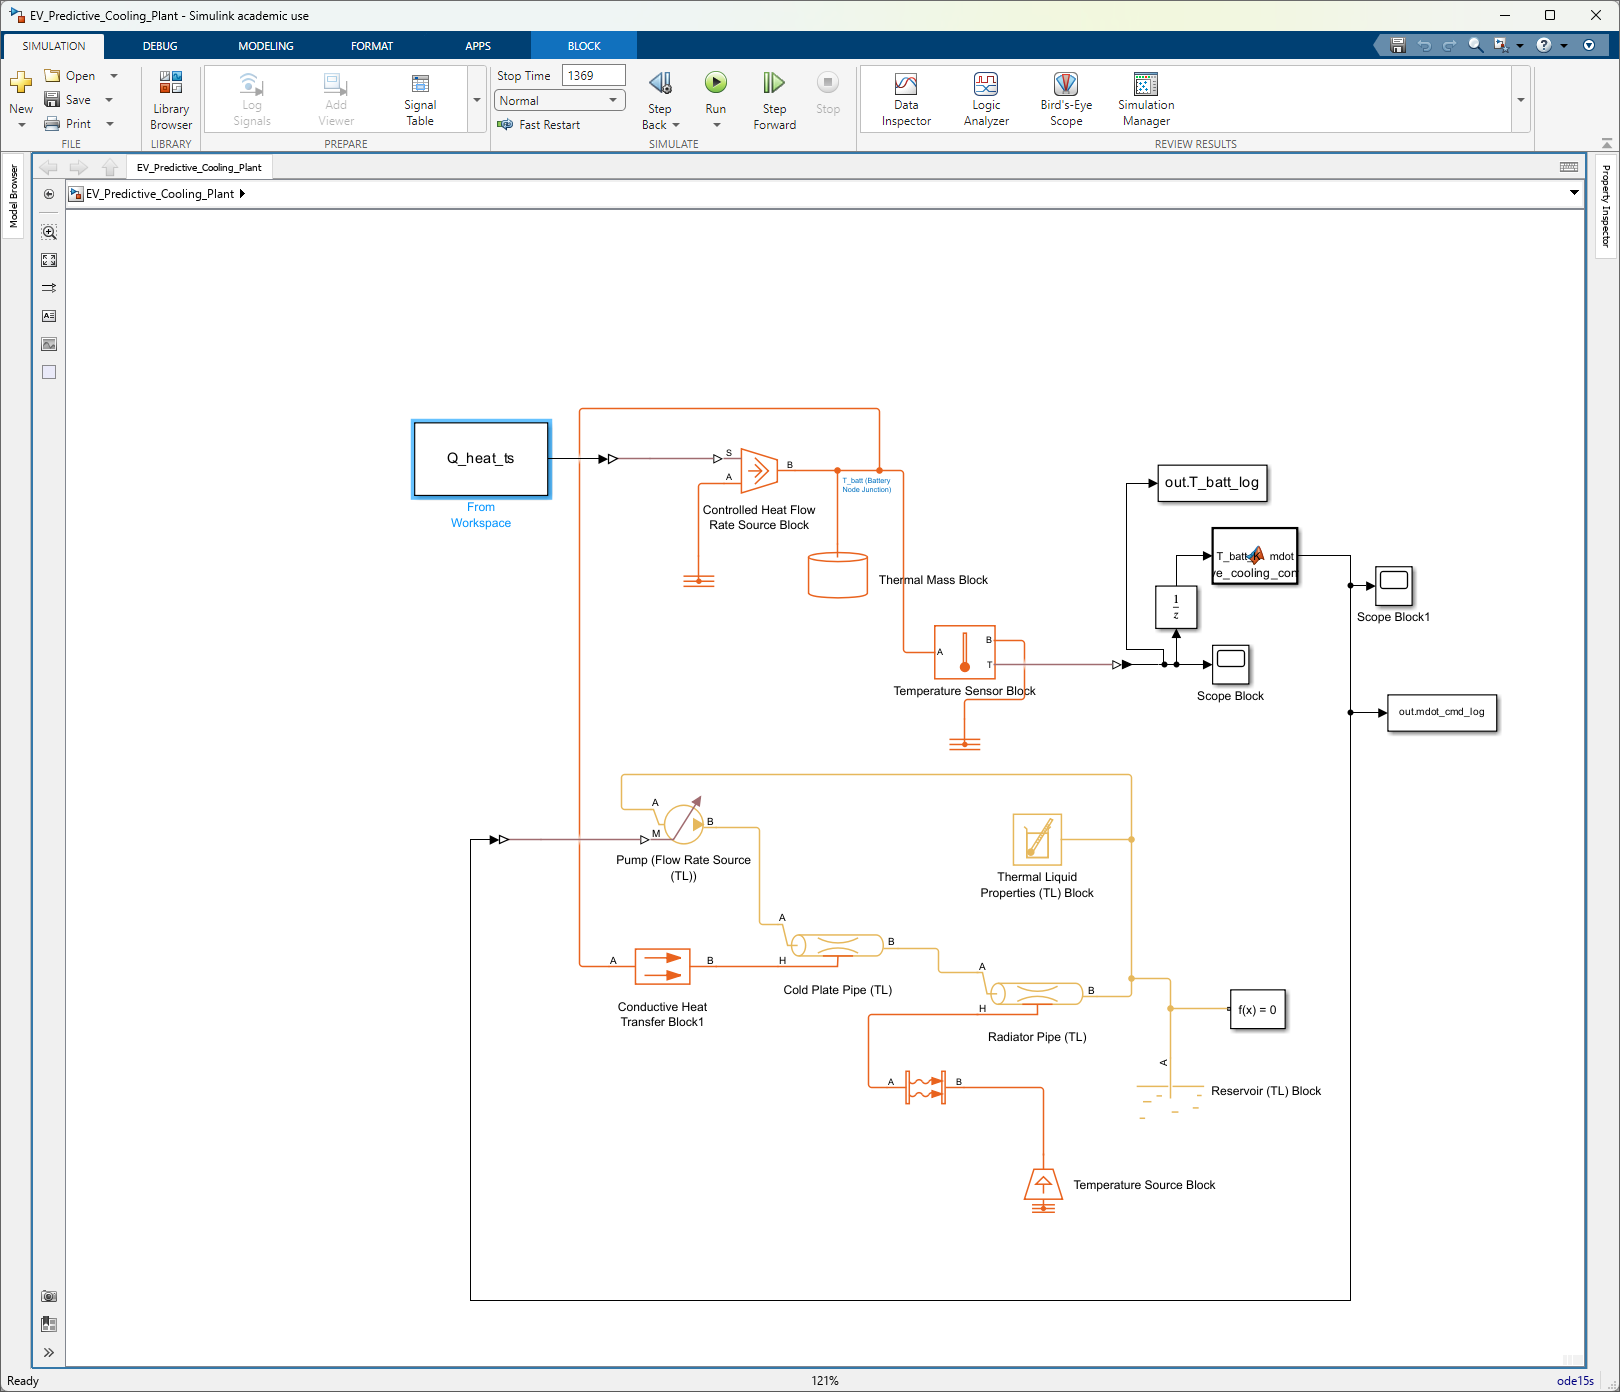
\includegraphics[width=0.95\linewidth]{EV_Predictive_Cooling_Plant_Simulink_Final_Model.png}
\caption{Simscape Fluids battery cooling plant: cold plate, coolant pump, radiator, reservoir, and thermal liquid properties network, with controller-commanded coolant flow.}
\label{fig:plant}
\end{figure}

Three physical plant variants were built: a closed-loop template, an open-loop \texttt{FixedHighFlow} variant with constant 0.05\,kg/s coolant flow used to isolate plant physics from controller behaviour during debugging, and a reactive-controller variant used for UDDS validation (Section~\ref{sec:results}). Isolating the plant from the controller in this way proved essential during development: when closed-loop temperature behaviour looked incorrect, the \texttt{FixedHighFlow} variant made it possible to confirm the thermal-fluid network itself was correct before re-introducing controller logic, narrowing the search space for the eventual bug (Section~\ref{sec:debug}).

\section{Mathematical Modeling}
\label{sec:model}

\subsection{Vehicle Longitudinal Dynamics}

The total traction force required at the wheels is the sum of rolling resistance, aerodynamic drag, and the force needed to accelerate the vehicle:
\begin{equation}
F_{total} = F_{rr} + F_{aero} + F_{acc}
\end{equation}
\begin{equation}
F_{rr} = mgC_{rr}, \qquad F_{aero} = \tfrac{1}{2}\rho C_d A v^2
\end{equation}
\begin{equation}
F_{acc} = m_{eq}a, \qquad m_{eq} = m(1+\delta)
\end{equation}
with $\delta = 0.08$ representing the rotational inertia of wheels, gears, and shafts, and acceleration clamped to $-4\le a\le 3$\,m/s$^2$ to remove differentiation noise from the drive-cycle speed trace.

\subsection{Wheel Power and Motor Torque--Speed Envelope}

\begin{equation}
P_{wheel} = \frac{F_{total}\,v}{\eta_{tire}}
\end{equation}
\begin{equation}
\omega_{base} = \frac{P_{motor,max}}{T_{motor,max}}
\end{equation}
The motor can only deliver as much torque as its constant-torque / constant-power envelope allows:
\begin{equation}
T_{avail} = \begin{cases}
T_{motor,max} & \omega \le \omega_{base} \\
P_{motor,max}/\omega & \omega > \omega_{base}
\end{cases}
\end{equation}
Regenerative braking is capped at $T_{regen,max}=120$\,Nm and disabled below $v_{min,regen}=1.5$\,m/s to represent motor back-EMF limitations at low speed.

\subsection{Battery Electrical Model}

Open-circuit voltage is obtained from an 11-point SOC--OCV lookup table, and internal resistance from a 2-D interpolant over SOC and temperature -- following the equivalent-circuit parameterisation methodology of Huria et al.~\cite{huria2012}, in which each circuit element is a function of SOC and temperature:
\begin{equation}
I_{batt} = \frac{P_{batt}}{V_{nom}}
\end{equation}
\begin{equation}
R_{int} = F_{R_{int}}(SOC, T_{batt})
\end{equation}
\begin{equation}
V_{batt} = V_{oc}(SOC) - I_{batt}R_{int}
\end{equation}
\begin{equation}
SOC_k = SOC_{k-1} - \frac{I_{batt}V_{nom}\Delta t}{3600\,C_{batt}}
\end{equation}

\subsection{Battery Heat Generation}

Heat generation is split into an irreversible ohmic term and a reversible entropic term, rather than the $I^2R$-only approximation common in simplified models:
\begin{equation}
Q_{ohmic} = I_{batt}^2 R_{int}
\end{equation}
\begin{equation}
Q_{entropic} = I_{batt}\,T_K\,\frac{dU}{dT}, \qquad \frac{dU}{dT} = -0.00022\ \text{V/K}
\end{equation}
\begin{equation}
Q_{heat} = Q_{ohmic} + Q_{entropic}
\end{equation}

\subsection{Lumped Battery Thermal Plant}

\begin{equation}
Q_{passive} = \frac{T_{batt}-T_{amb}}{R_{th}}
\end{equation}
\begin{equation}
\frac{dT_{batt}}{dt} = \frac{Q_{heat}-Q_{passive}-Q_{cooling}}{C_{th}}
\end{equation}
with $C_{th}=45000$\,J/K and $R_{th}=1.5$\,K/W. The Simscape Fluids plant (Section~\ref{sec:arch}) replaces this lumped equation with a physical Thermal Mass + Cold Plate + Radiator network for validation.

\subsection{Controller 1: Reactive Baseline (Hysteresis)}

\begin{equation}
Q_{cooling} = \begin{cases}
Q_{cooling,max} & T_{batt}\ge T_{on}\ (35^{\circ}\text{C}) \\
0 & T_{batt}\le T_{off}\ (32^{\circ}\text{C}) \\
\text{unchanged} & \text{otherwise}
\end{cases}
\end{equation}
This is a conventional thermostat: it cannot act until the battery has already crossed the trip point, and it cannot anticipate that heat generation is about to rise or fall.

\subsection{Controller 2: Predictive Lookahead Controller}

The predictive controller pre-cools \emph{before} the temperature threshold is reached, using three forecast signals: charger-proximity telematics $d_{charger}=s_{charger}-s_{route}(t)$, throttle-demand lookahead $\hat{\theta}_{throttle}=\max\big(\theta_{throttle}(t..t{+}15\text{s})\big)$, and a heat-generation forecast
\begin{equation}
\overline{Q}_{pred} = \text{mean}\big(Q_{heat}(t..t{+}H_p)\big), \qquad H_p = 120\ \text{s}.
\end{equation}
When the battery is at or above the target setpoint, the requested cooling power is
\begin{equation}
Q_{req} = \overline{Q}_{pred} + \frac{C_{th}\,(T_{batt}-T_{set})}{\tau_{control}}
\end{equation}
and the commanded cooling power follows the decision logic
\begin{equation}
Q_{cooling} = \begin{cases}
Q_{cooling,max} & \text{charger flag}\wedge T_{batt}{>}28^{\circ}\text{C} \\
0.75\,Q_{cooling,max} & \hat{\theta}_{throttle}{>}50\wedge T_{batt}{>}29^{\circ}\text{C} \\
\text{clamp}(Q_{req},0,Q_{cooling,max}) & T_{batt}\ge T_{set} \\
0 & \text{otherwise.}
\end{cases}
\end{equation}
This directly implements the brief's request for a controller informed by charge rate, throttle position, and location data.

\subsection{Controller 3: Constrained Nonlinear MPC}

A receding-horizon MPC solves, at every timestep, for the cooling-power sequence over the horizon $H_p$ that minimises a weighted cost
\begin{equation}
J = \sum_{k=1}^{H_p} w_T\,e_T(k)^2 + w_E\,u(k)^2 + w_{dU}\,\Delta u(k)^2,
\end{equation}
where the tracking error and control-rate terms are
\begin{equation}
e_T(k) = T_{pred}(k)-T_{set}, \qquad \Delta u(k) = u(k)-u(k-1),
\end{equation}
subject to the thermal-plant dynamics evaluated across the horizon,
\begin{align}
T_{pred}(k{+}1) = {}& T_{pred}(k) \notag \\
& + \frac{\Delta t}{C_{th}}\left(Q_{heat}(k)-\frac{T_{pred}(k)-T_{amb}(k)}{R_{th}}-u(k)\right),
\end{align}
and to the actuator and safety bounds
\begin{equation}
0\le u(k)\le Q_{cooling,max} \qquad \forall k\in\{1,\dots,H_p\},
\end{equation}
\begin{equation}
T_{pred}(k)\le T_{max}\ (35^{\circ}\text{C}) \qquad \forall k\in\{1,\dots,H_p\}.
\end{equation}
The problem is solved with \texttt{fmincon} (SQP algorithm, warm-started from the previous solution), applying only the first control action of each solve in standard receding-horizon fashion. The energy weight ($w_E=10^{-5}$) and slew-rate weight ($w_{dU}=10^{-3}$) trade cooling-energy use and actuator wear against tracking accuracy.

\subsection{SOC Estimation via Kalman Filter}

Prediction (coulomb counting):
\begin{equation}
\widehat{SOC}_{k|k-1} = \widehat{SOC}_{k-1} - \frac{I_{batt}(k)\,\Delta t}{3600\,C_{Ah}}
\end{equation}
\begin{equation}
P_{k|k-1} = P_{k-1} + Q_{process}
\end{equation}
Update (voltage correction):
\begin{equation}
K = \frac{P_{k|k-1}H}{H\,P_{k|k-1}H + R}
\end{equation}
\begin{equation}
\widehat{SOC}_k = \widehat{SOC}_{k|k-1} + K\big(V_{meas}(k)-V_{oc,pred}\big)
\end{equation}
with sensitivity $H=100$, measurement noise $R=0.5$, and process noise $Q_{process}=10^{-6}$, approximating the voltage-based SOC estimation used in a real battery management system.

\subsection{Battery Aging (Arrhenius SEI Growth)}

Instantaneous capacity-fade rate is modelled with an Arrhenius temperature dependence:
\begin{equation}
k_{deg}(T) = A_{pre}\exp\!\left(\frac{-E_a}{R_{gas}T_K}\right), \qquad E_a = 31700\ \text{J/mol}
\end{equation}
\begin{equation}
\text{aging} = \int_0^{t_{end}} k_{deg}\big(T(t)\big)\,dt.
\end{equation}
Relative life extension of a controller versus the reactive baseline is $(\text{aging}_{base}-\text{aging}_x)/\text{aging}_{base}$, and additional driving range unlocked by spending less energy on cooling is $(E_{base}-E_x)/\text{specific consumption (Wh/km)}$.

\section{Implementation Methodology}
\label{sec:impl}

Table~\ref{tab:files} summarises the repository's key MATLAB and Simulink artifacts, and Table~\ref{tab:params} lists the controller parameter values used throughout Sections~\ref{sec:model} and~\ref{sec:results}.

\begin{table}[t]
\centering
\caption{Key implementation files}
\label{tab:files}
\small
\begin{tabular}{@{}p{0.46\linewidth}p{0.44\linewidth}@{}}
\toprule
\textbf{File} & \textbf{Role} \\
\midrule
\texttt{\seqsplit{ev\_eneergy\_model\_realistic\_predictive\_cooling.m}} & UDDS-based powertrain + battery model; generates \texttt{\seqsplit{EV\_Thermal\_Inputs.mat}} \\
\addlinespace
\texttt{\seqsplit{Dynamic\_Loads.m}} & Synthetic 2000\,s multi-phase mission; implements and benchmarks all three controllers plus Kalman SOC estimator \\
\addlinespace
\texttt{\seqsplit{EV\_Predictive\_Cooling\_Plant\_Reactive.slx}} & Reactive baseline wired into Simscape Fluids plant \\
\addlinespace
\texttt{\seqsplit{EV\_Predictive\_Cooling\_Plant\_FixedHighFlow.slx}} & Open-loop constant-flow reference plant \\
\addlinespace
\texttt{\seqsplit{build\_predictive\_mpc\_models.m}} & Clones reactive plant; wires in \texttt{matlab.System} predictive/MPC controllers \\
\addlinespace
\texttt{\seqsplit{run\_project.m}} & Single entry point; runs full pipeline end-to-end \\
\bottomrule
\end{tabular}
\end{table}

\begin{table}[t]
\centering
\caption{Controller parameters (stress scenario)}
\label{tab:params}
\small
\begin{tabular}{@{}lll@{}}
\toprule
\textbf{Controller} & \textbf{Parameter} & \textbf{Value} \\
\midrule
Reactive & $T_{on}$ / $T_{off}$ & 35\textdegree C / 32\textdegree C \\
Reactive & $Q_{cooling,max}$ & 2000\,W \\
Predictive & $H_p$ & 120\,s \\
Predictive & $T_{pre,target}$ / $T_{set}$ & 28\textdegree C / 32\textdegree C \\
Predictive & $\tau_{control}$ & 30\,s \\
MPC & $H_p$ / $T_{set}$ / $T_{max}$ & 120\,s / 32\textdegree C / 35\textdegree C \\
MPC & $w_T$ / $w_E$ / $w_{dU}$ & 100 / $10^{-5}$ / $10^{-3}$ \\
\bottomrule
\end{tabular}
\end{table}

Each script is designed to run independently with no manual intervention: \texttt{run\_project.m} regenerates the UDDS-based thermal input signals, runs the MATLAB-only controller comparison, simulates the reactive Simscape Fluids plant, and finally builds and simulates the predictive/MPC Simscape plant variants, reporting which stages were skipped and why if a required product (Simulink, Simscape Fluids, Optimization Toolbox) is unavailable, rather than failing silently.

\section{Simulation Results}
\label{sec:results}

Two independent result sets are reported, from different plants and scenarios, kept separate deliberately because they carry different evidentiary status.

\subsection{Simulink Reactive-Baseline Diagnostics (UDDS Scenario)}

Re-running \texttt{\seqsplit{EV\_Predictive\_Cooling\_Plant\_Reactive.slx}} on the real EPA UDDS drive cycle (1369\,s) shows the battery temperature rising only from approximately 300.0\,K (26.85\textdegree C) to 300.3\,K ($\sim$27.2\textdegree C) -- Fig.~\ref{fig:udds_temp} -- with the reactive controller's 32\textdegree C threshold never triggered, so coolant flow remains at its minimum baseline value throughout (Fig.~\ref{fig:udds_flow}). This confirms the Simscape Fluids plant and reactive controller behave physically sensibly on real urban driving, though this scenario alone is mild enough that it does not exercise active cooling or a thermal safety margin -- which is precisely why the more demanding stress scenario of Section~\ref{sec:results}B is needed to evaluate the predictive and MPC controllers meaningfully.

\begin{figure}[t]
\centering
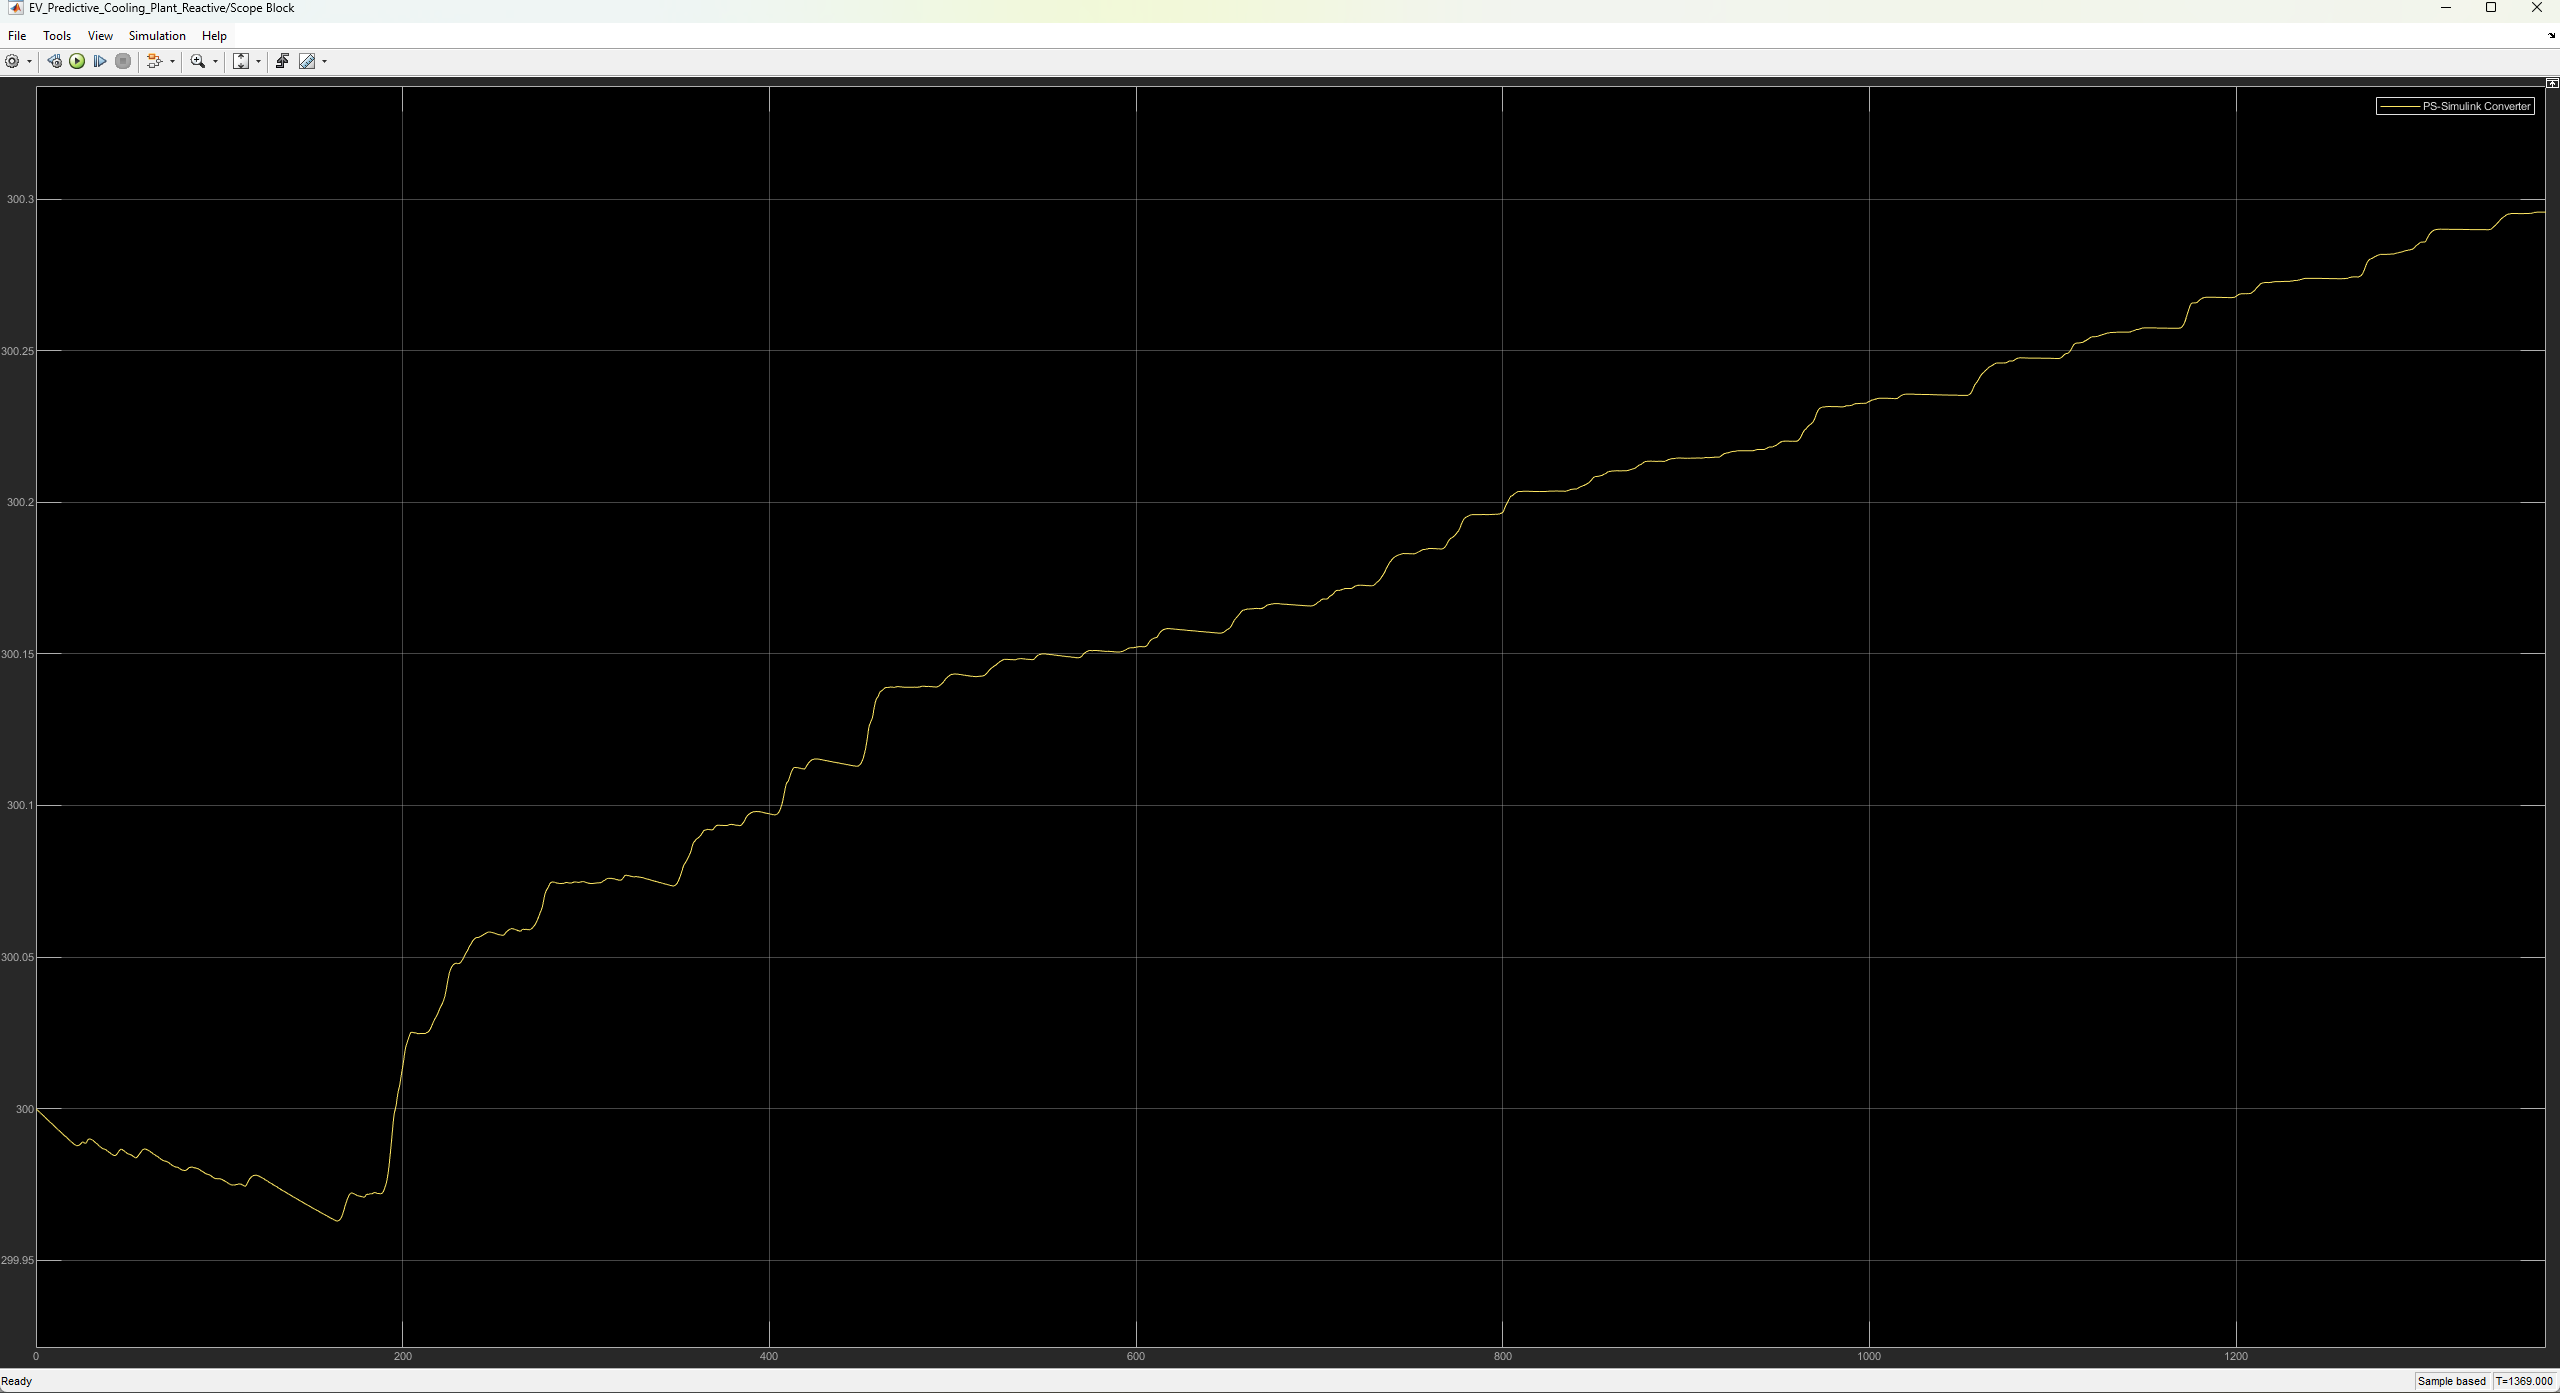
\includegraphics[width=0.95\linewidth]{Reactive_Simscape_Battery_Temp_UDDS.png}
\caption{Battery temperature (K) over the 1369\,s UDDS drive cycle, reactive-controlled Simscape Fluids plant.}
\label{fig:udds_temp}
\end{figure}

\begin{figure}[t]
\centering
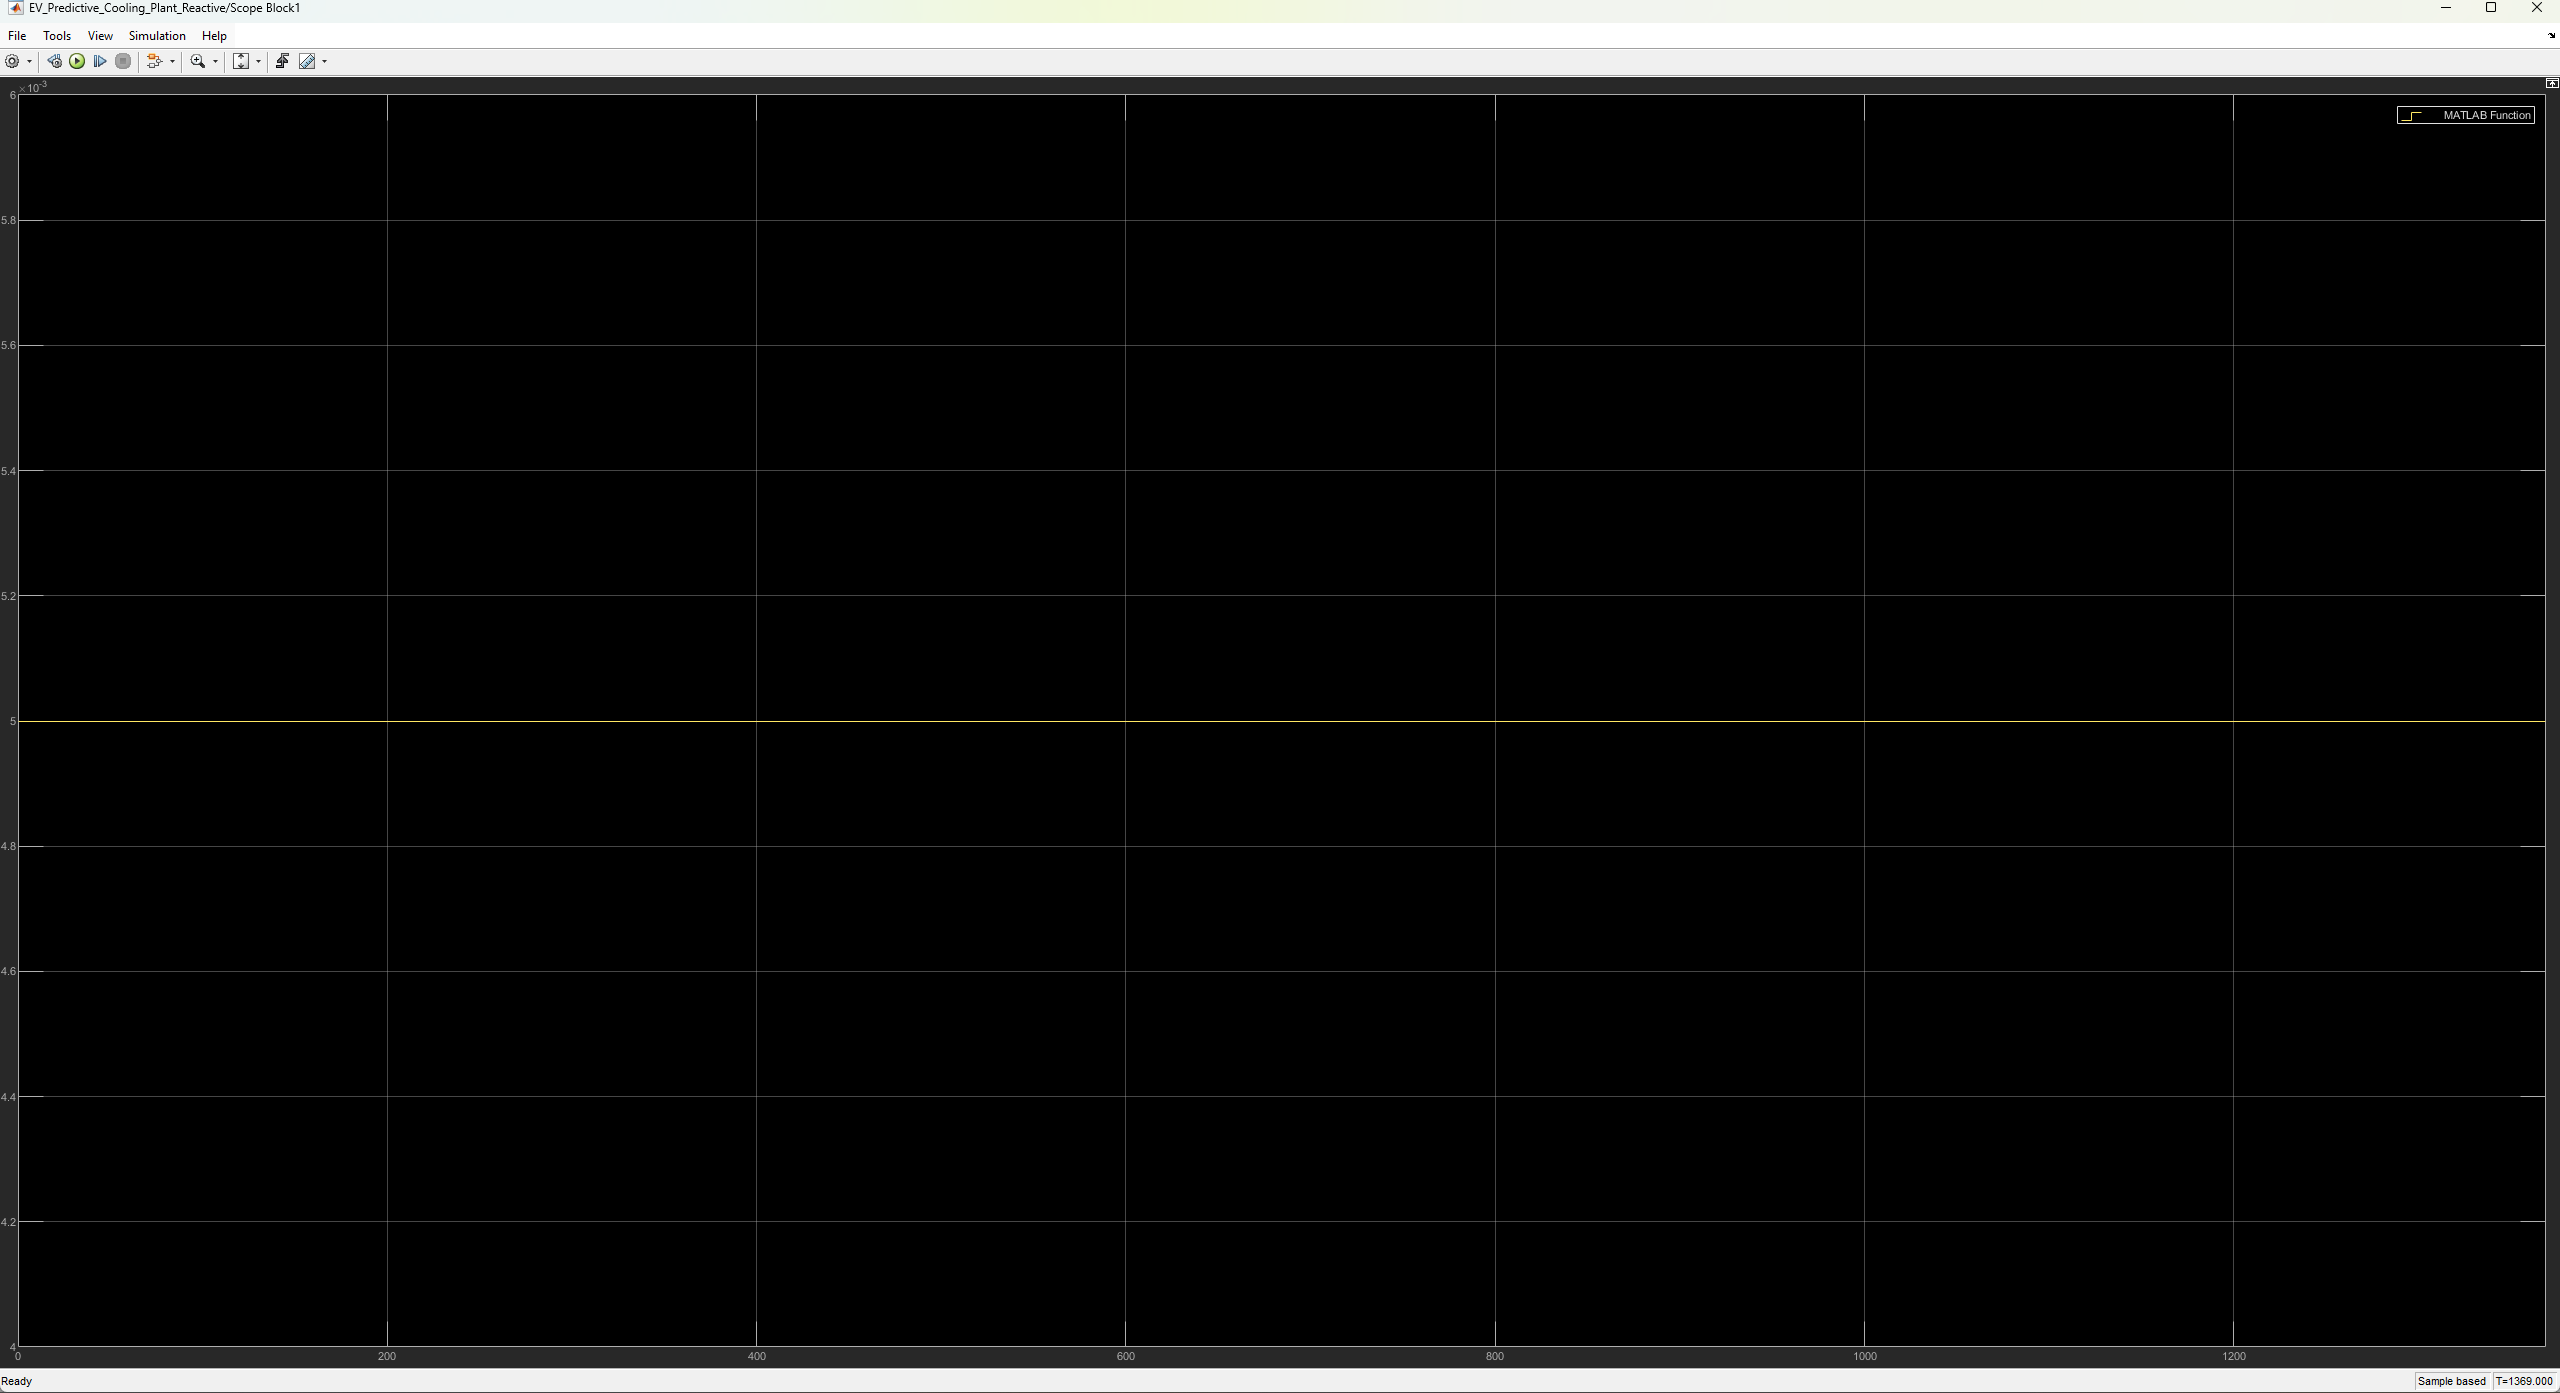
\includegraphics[width=0.95\linewidth]{Reactive_Simscape_Coolant_Flow_UDDS.png}
\caption{Commanded coolant mass flow rate over the UDDS cycle; the reactive threshold is never triggered, so flow stays at its minimum baseline value.}
\label{fig:udds_flow}
\end{figure}

\subsection{MATLAB-Based Multi-Controller Comparison (Stress Scenario)}
\label{sec:results-stress}

\texttt{Dynamic\_Loads.m} runs the uncooled plant and all three controllers over a 2000\,s aggressive-drive $\rightarrow$ fast-charge $\rightarrow$ soak scenario (Fig.~\ref{fig:loadprofile}), combining driving heat, a 300\,A DC fast-charge heat surge, and an ambient ramp from 25\textdegree C to 38\textdegree C. This scenario is deliberately more demanding than the UDDS case: it is constructed to stress both the drive-induced and charge-induced heat pathways simultaneously, which is the operating regime in which a reactive controller's inherent lag is most costly. Table~\ref{tab:benchmark} reports the captured console output from a full run.

\begin{figure}[t]
\centering
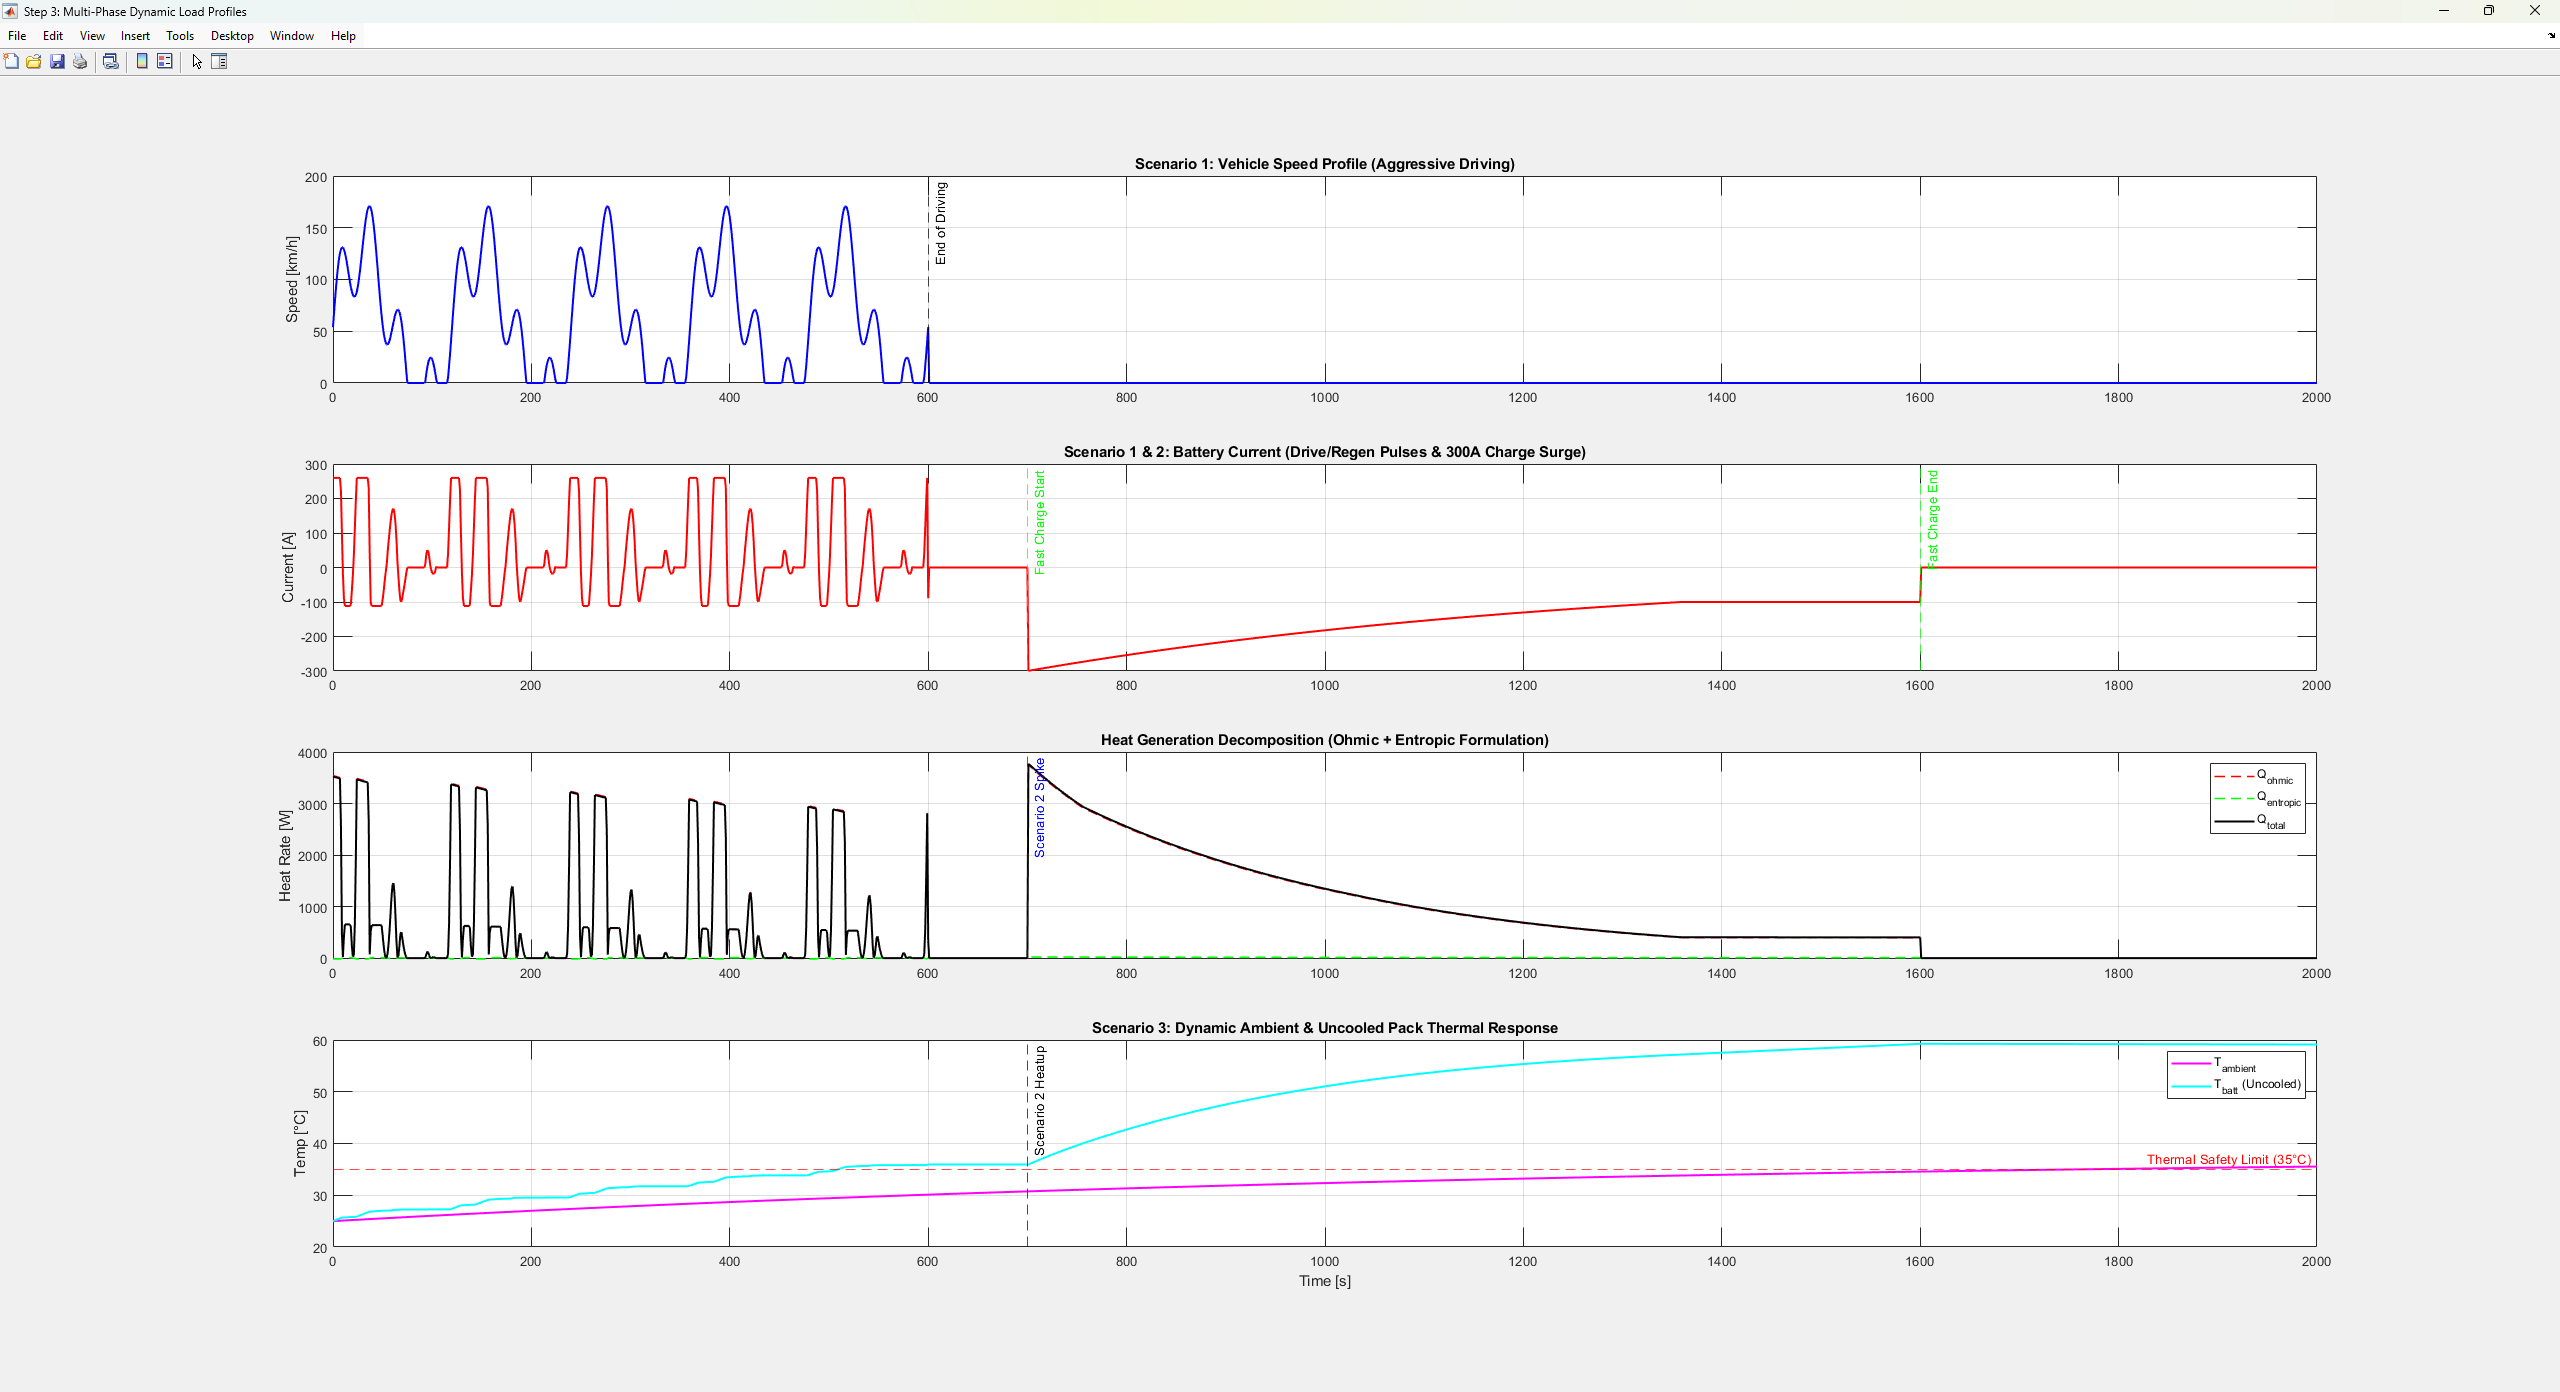
\includegraphics[width=0.95\linewidth]{Multi-Phase_Dynamic_Load_Profiles.png}
\caption{Stress scenario: vehicle speed, battery current, heat-generation decomposition, and dynamic ambient/uncooled thermal response.}
\label{fig:loadprofile}
\end{figure}

\begin{table}[t]
\centering
\caption{Comprehensive controller benchmark, 2000\,s stress scenario}
\label{tab:benchmark}
\small
\begin{tabular}{@{}lrrrr@{}}
\toprule
\textbf{Metric} & \textbf{Uncooled} & \textbf{Reactive} & \textbf{Predictive} & \textbf{MPC} \\
\midrule
Peak temp (\textdegree C) & 59.27 & 36.58 & 33.60 & 33.61 \\
Time $>$35\textdegree C (s) & 1491 & 313 & \textbf{0} & \textbf{0} \\
Time $>$32\textdegree C (s) & 1639 & 1634 & 1261 & 1426 \\
Chiller energy (Wh) & -- & 142.14 & 157.84 & 160.97 \\
Energy vs.\ baseline (\%) & -- & baseline & $-11.05$ & $-13.25$ \\
Actuator chatter (W/s) & -- & 6.00 & 23.00 & 4.41 \\
Aging reduction (\%) & -- & baseline & 7.71 & 5.18 \\
Range impact (km) & -- & 0.000 & $-0.070$ & $-0.084$ \\
\bottomrule
\end{tabular}
\end{table}

Figure~\ref{fig:benchmark} shows temperature, cumulative cooling energy, and Arrhenius aging rate together across all four cases. The predictive and MPC controllers eliminate every safety-threshold excursion, at the cost of higher cumulative cooling energy than the reactive baseline -- a genuine trade-off: forecast-aware control spends energy proactively ahead of the fast-charge and throttle-spike events, converting that spend into fewer and shorter safety excursions and lower modelled battery aging exposure.

\begin{figure}[t]
\centering
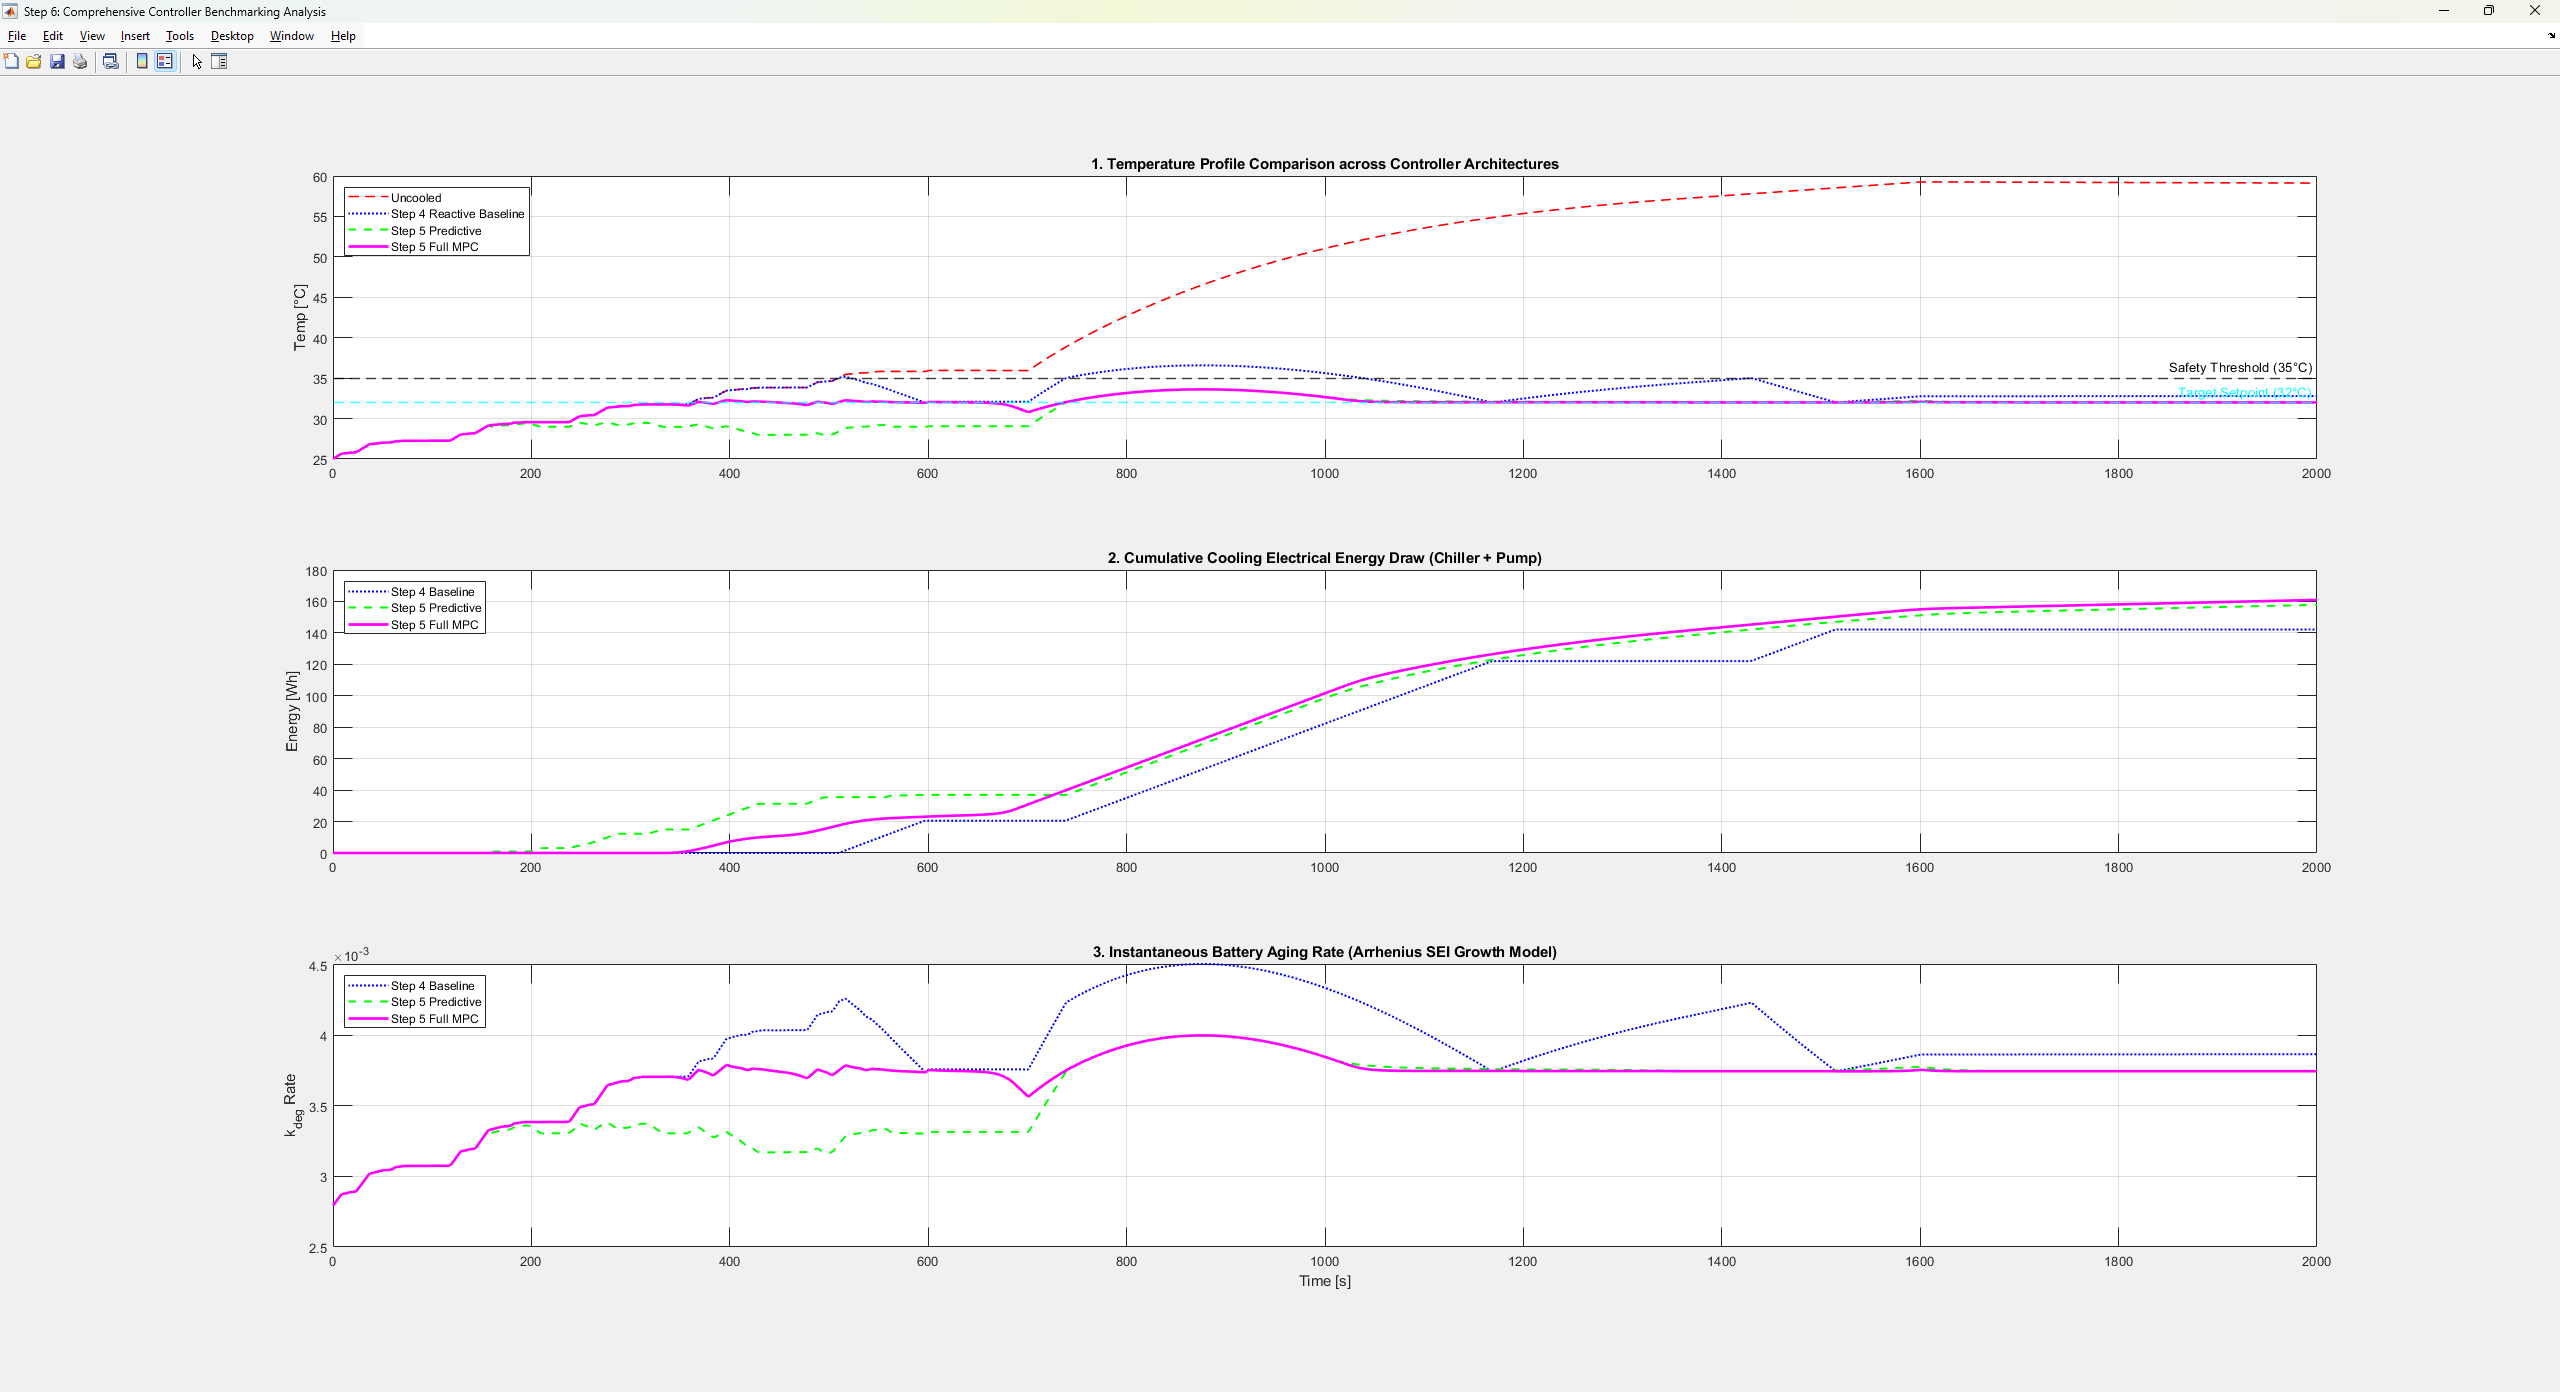
\includegraphics[width=0.95\linewidth]{Comprehensive_Controller_Benchmarking_Analysis.png}
\caption{Temperature, cumulative cooling energy, and Arrhenius battery-aging rate across the uncooled, reactive, predictive, and MPC cases.}
\label{fig:benchmark}
\end{figure}

\subsection{Predictive vs.\ Reactive and Full MPC Comparisons}

Figures~\ref{fig:predvsreact} and~\ref{fig:mpc} isolate the predictive-vs-reactive and full-MPC comparisons respectively. The predictive controller pre-cools ahead of both throttle spikes and the fast-charge event, holding the pack in a 28--31\textdegree C band before the demand arrives; the MPC controller tracks the 32\textdegree C setpoint the tightest of the three and has the lowest actuator chatter (4.41\,W/s) because its cost function explicitly penalises slew rate, whereas the predictive controller's simpler bang-bang pre-cool logic produces the highest chatter (23.00\,W/s).

\begin{figure}[t]
\centering
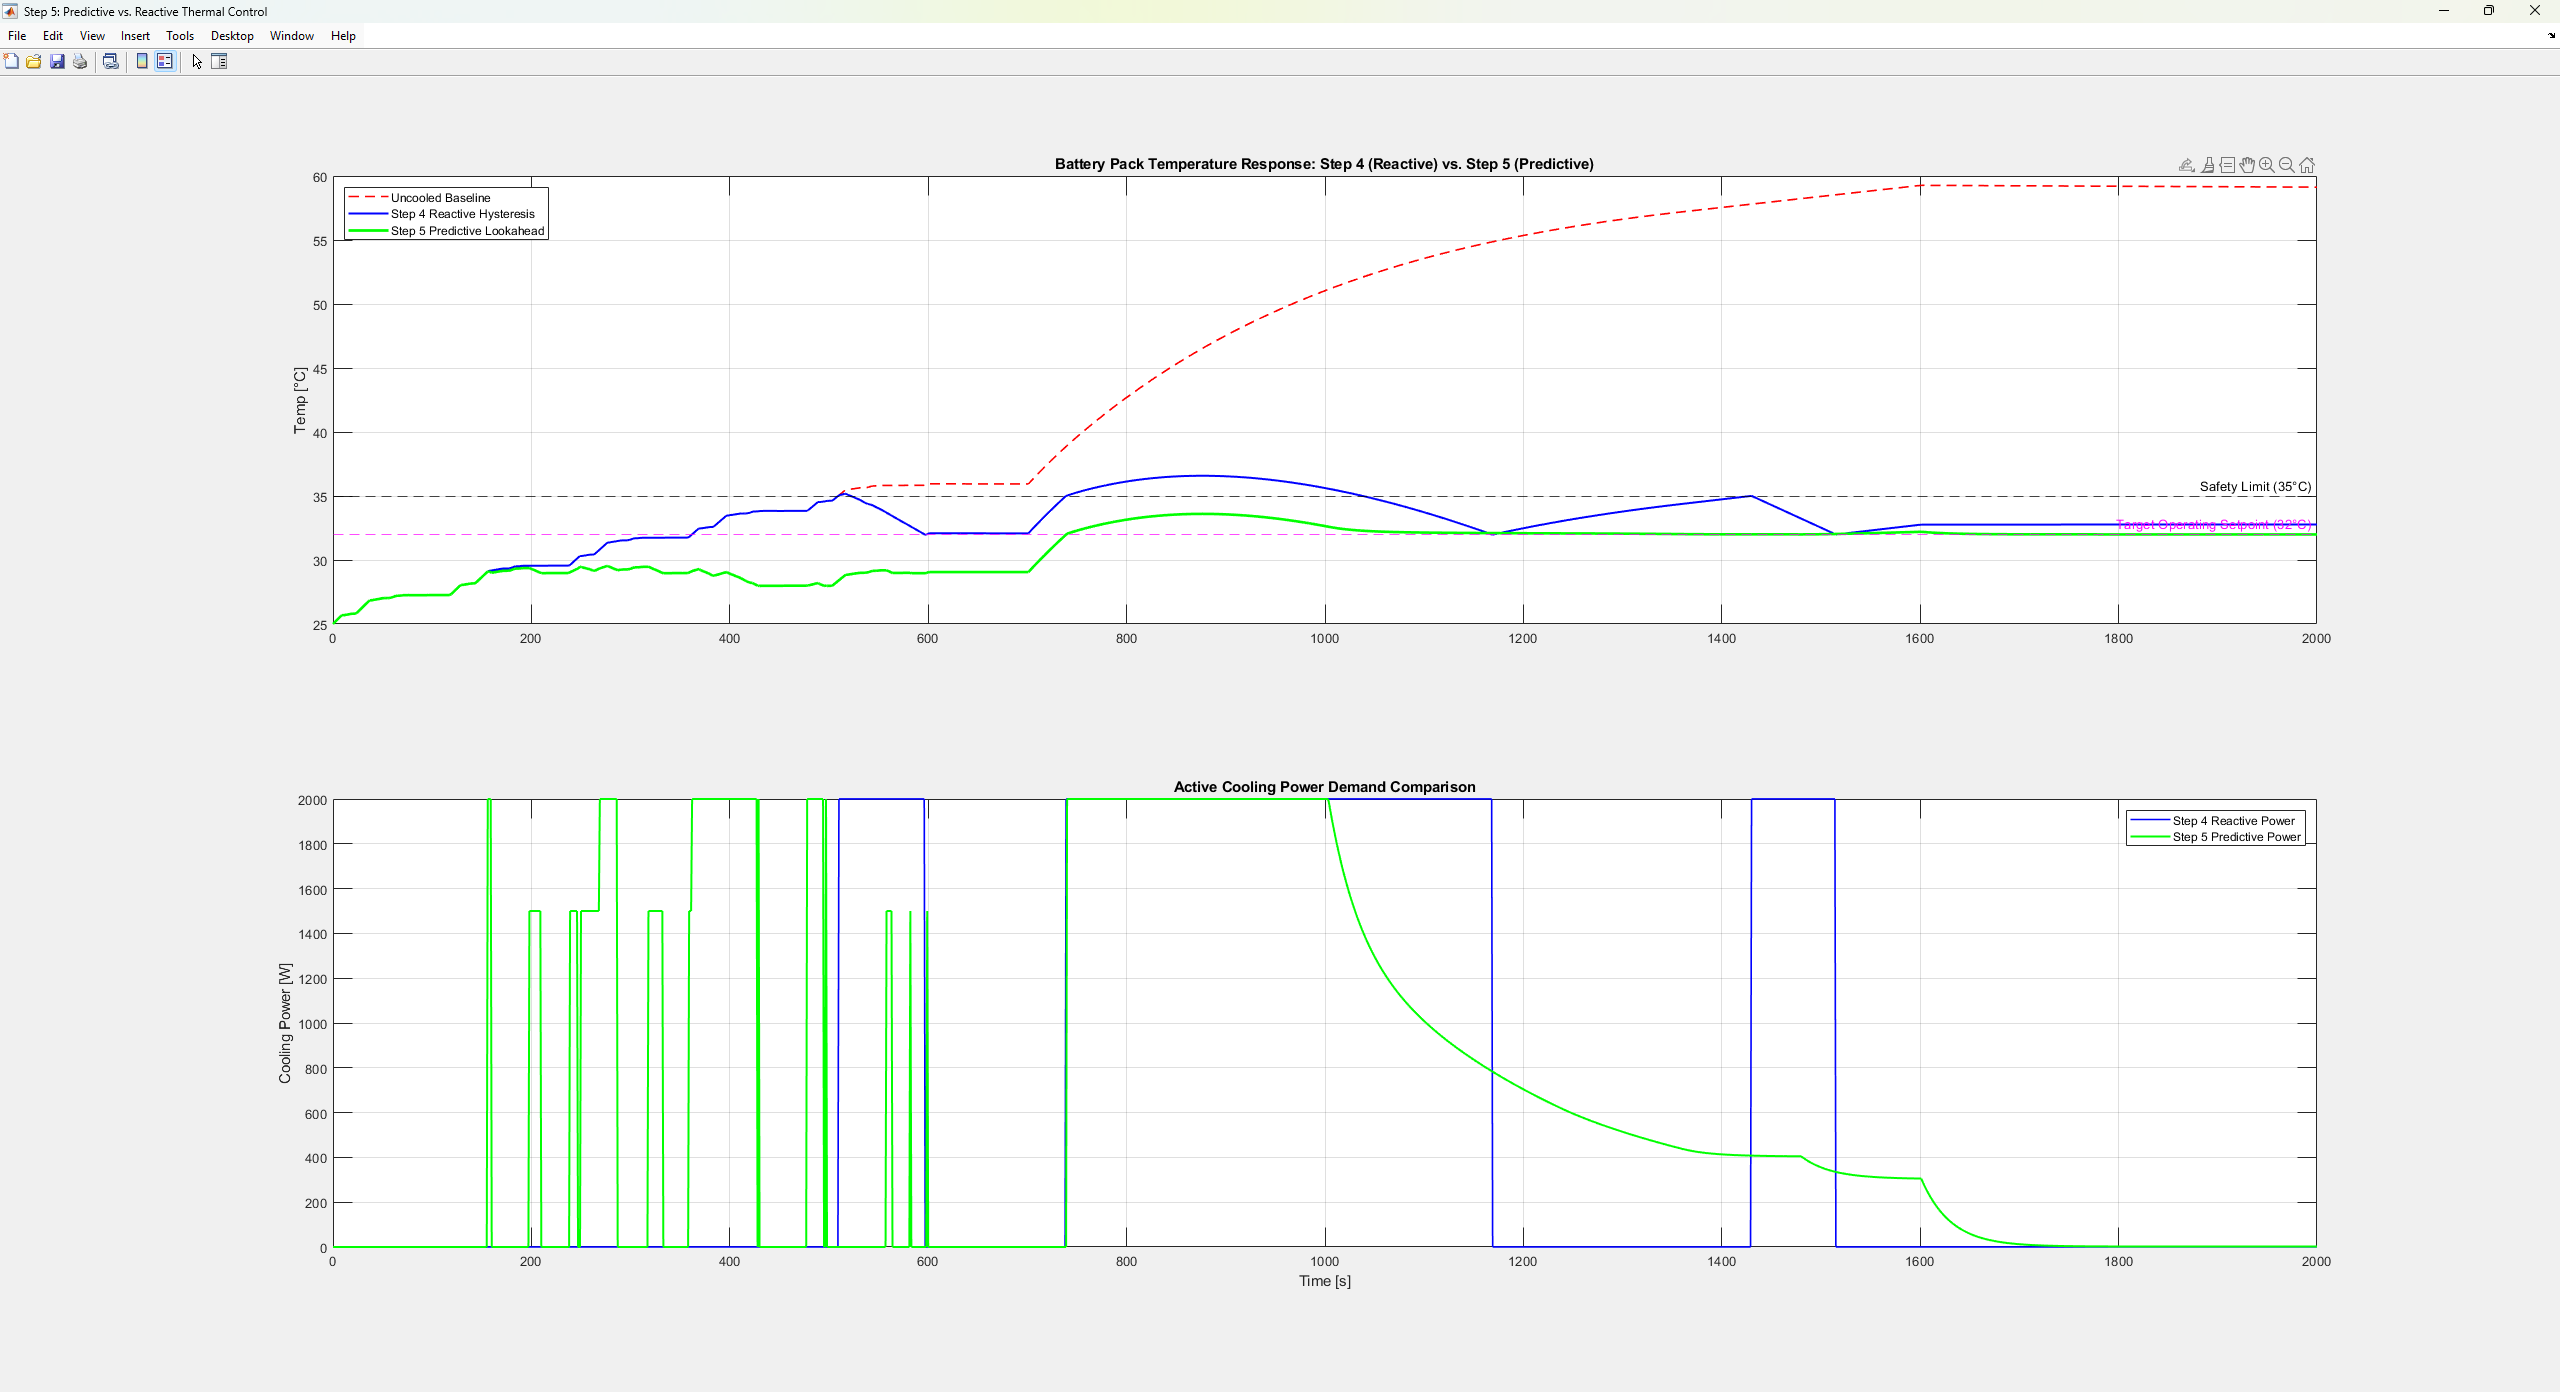
\includegraphics[width=0.95\linewidth]{Predictive_vs_Reactive_Thermal_Control.png}
\caption{Battery temperature and active cooling power: reactive hysteresis vs.\ predictive lookahead controller.}
\label{fig:predvsreact}
\end{figure}

\begin{figure}[t]
\centering
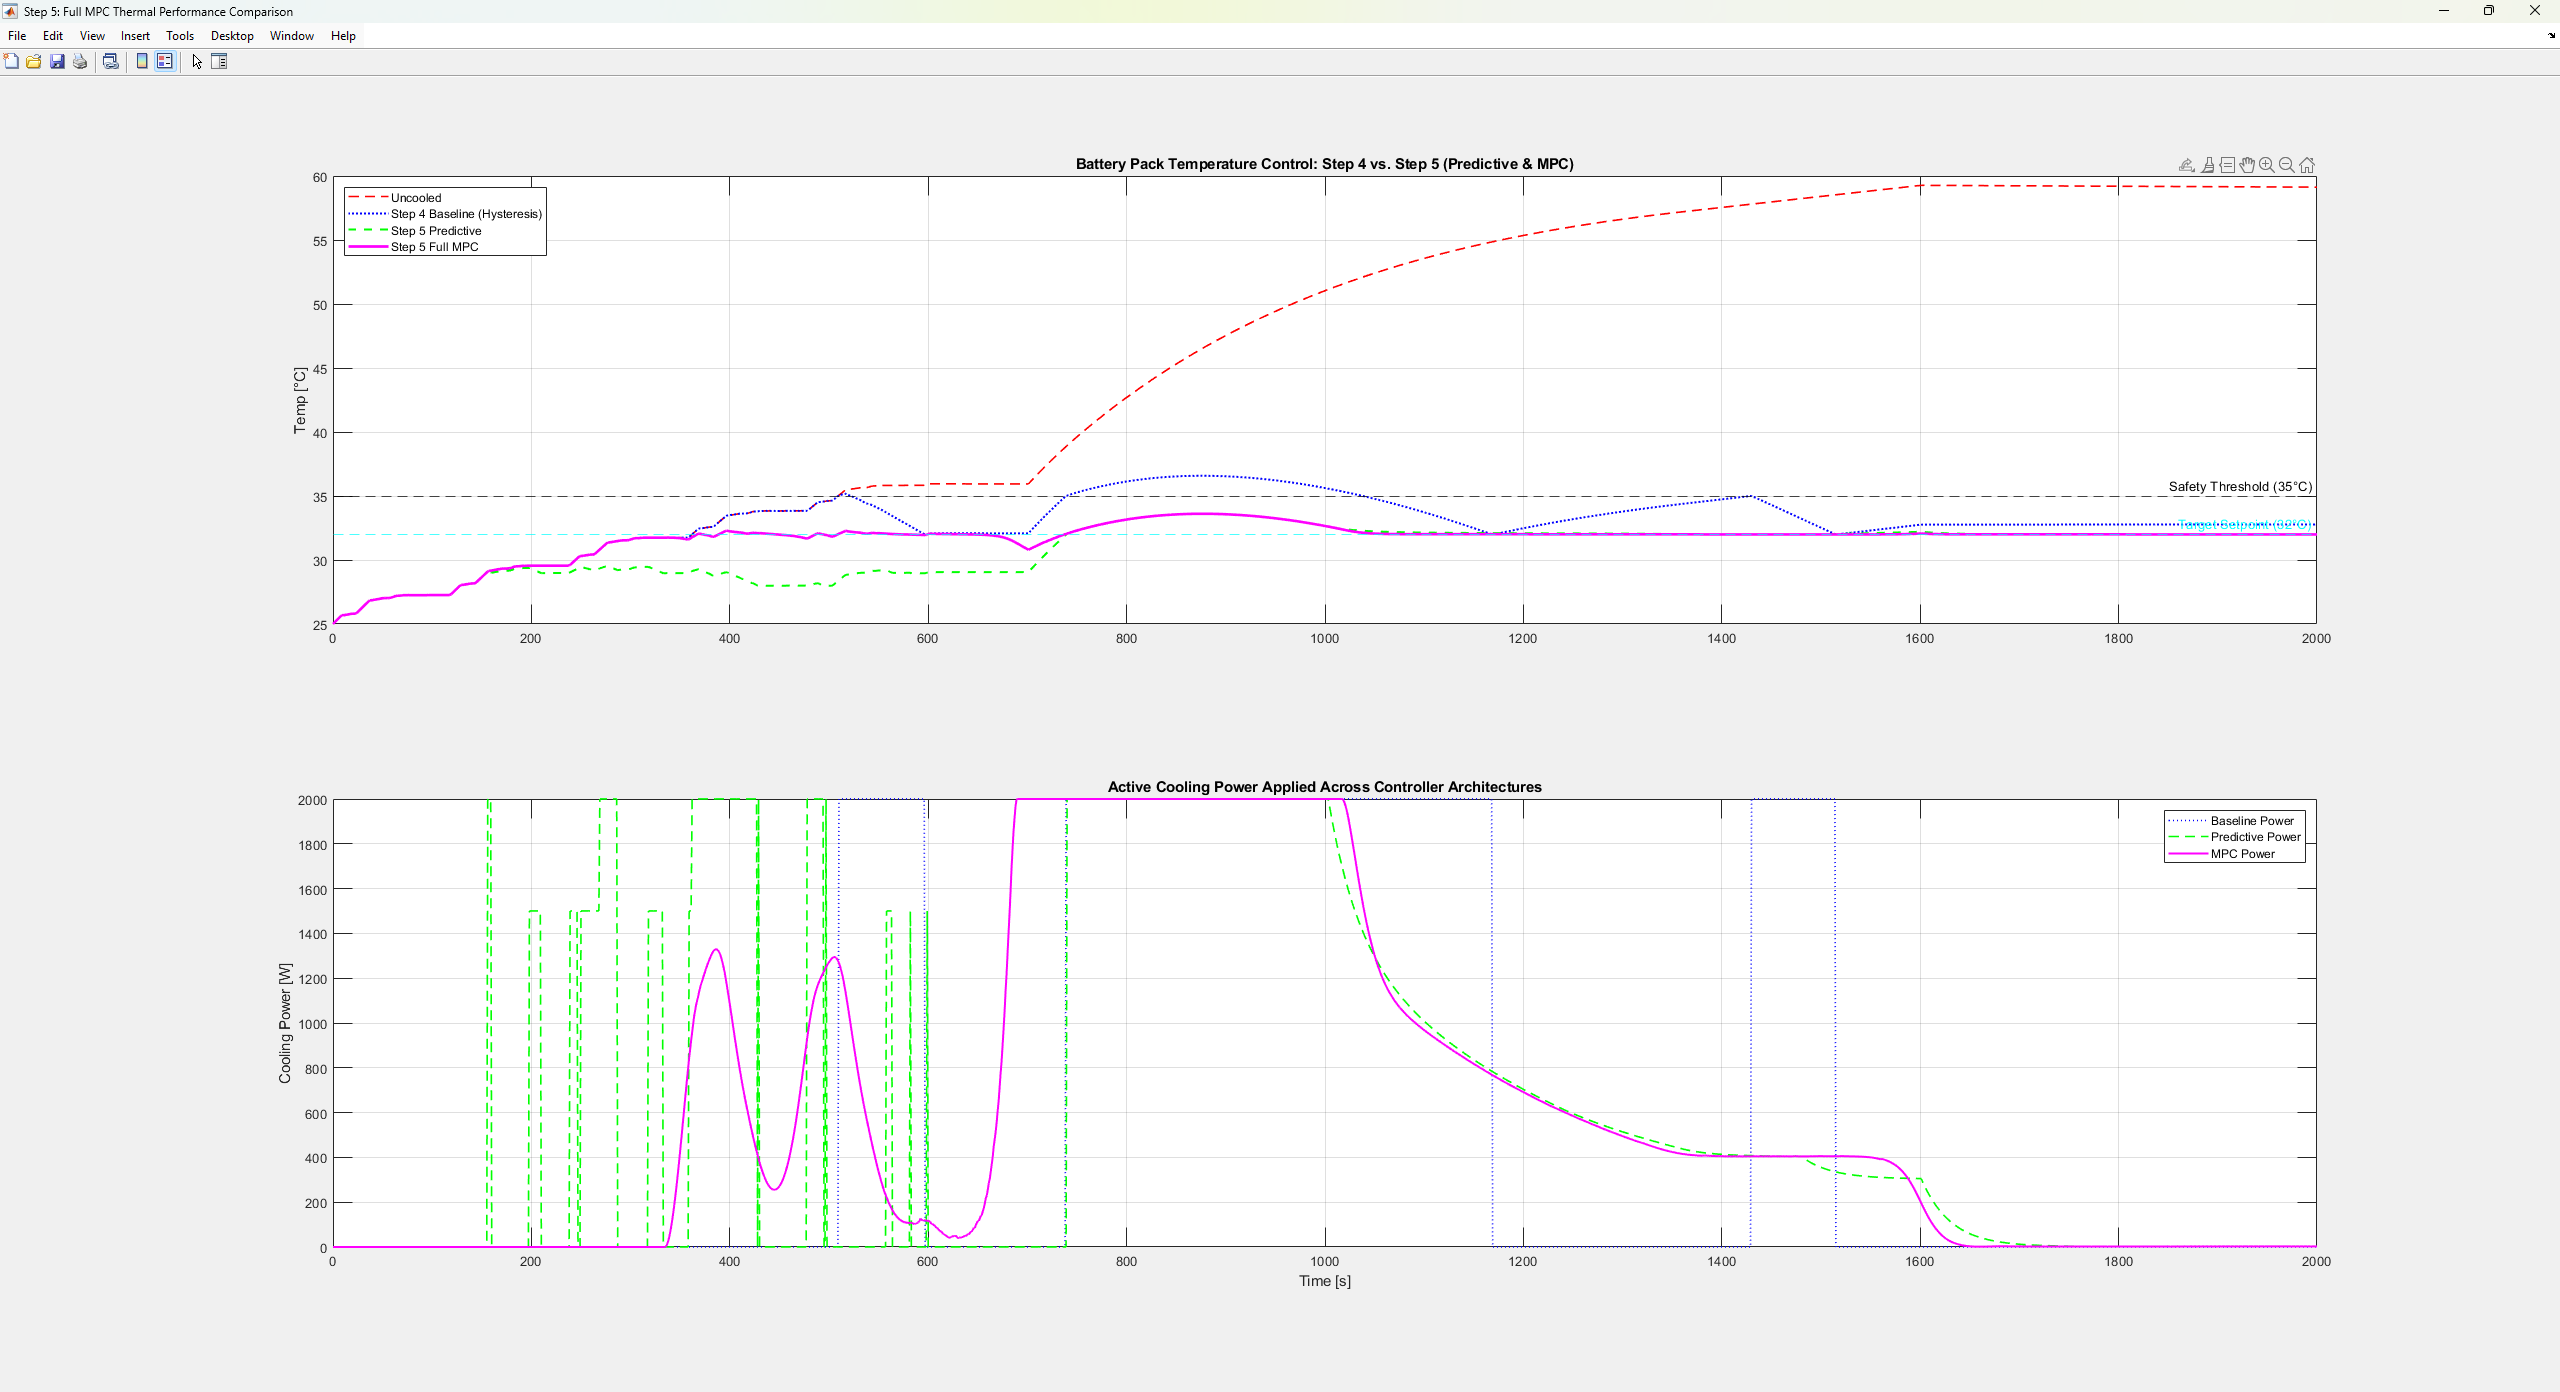
\includegraphics[width=0.95\linewidth]{Full_MPC_Thermal_Performance_Comparison.png}
\caption{Battery temperature and active cooling power across all three controller architectures, including full nonlinear MPC.}
\label{fig:mpc}
\end{figure}

\subsection{Electrical and SOC Tracking}

Figure~\ref{fig:soc} shows terminal voltage and Kalman-filter SOC tracking against true SOC over the stress scenario, confirming the estimator remains accurate through the drive, regenerative-braking, and fast-charge phases despite injected measurement noise, which supports its use as the SOC input each controller implicitly relies upon for capacity-normalised coulomb counting.

\begin{figure}[t]
\centering
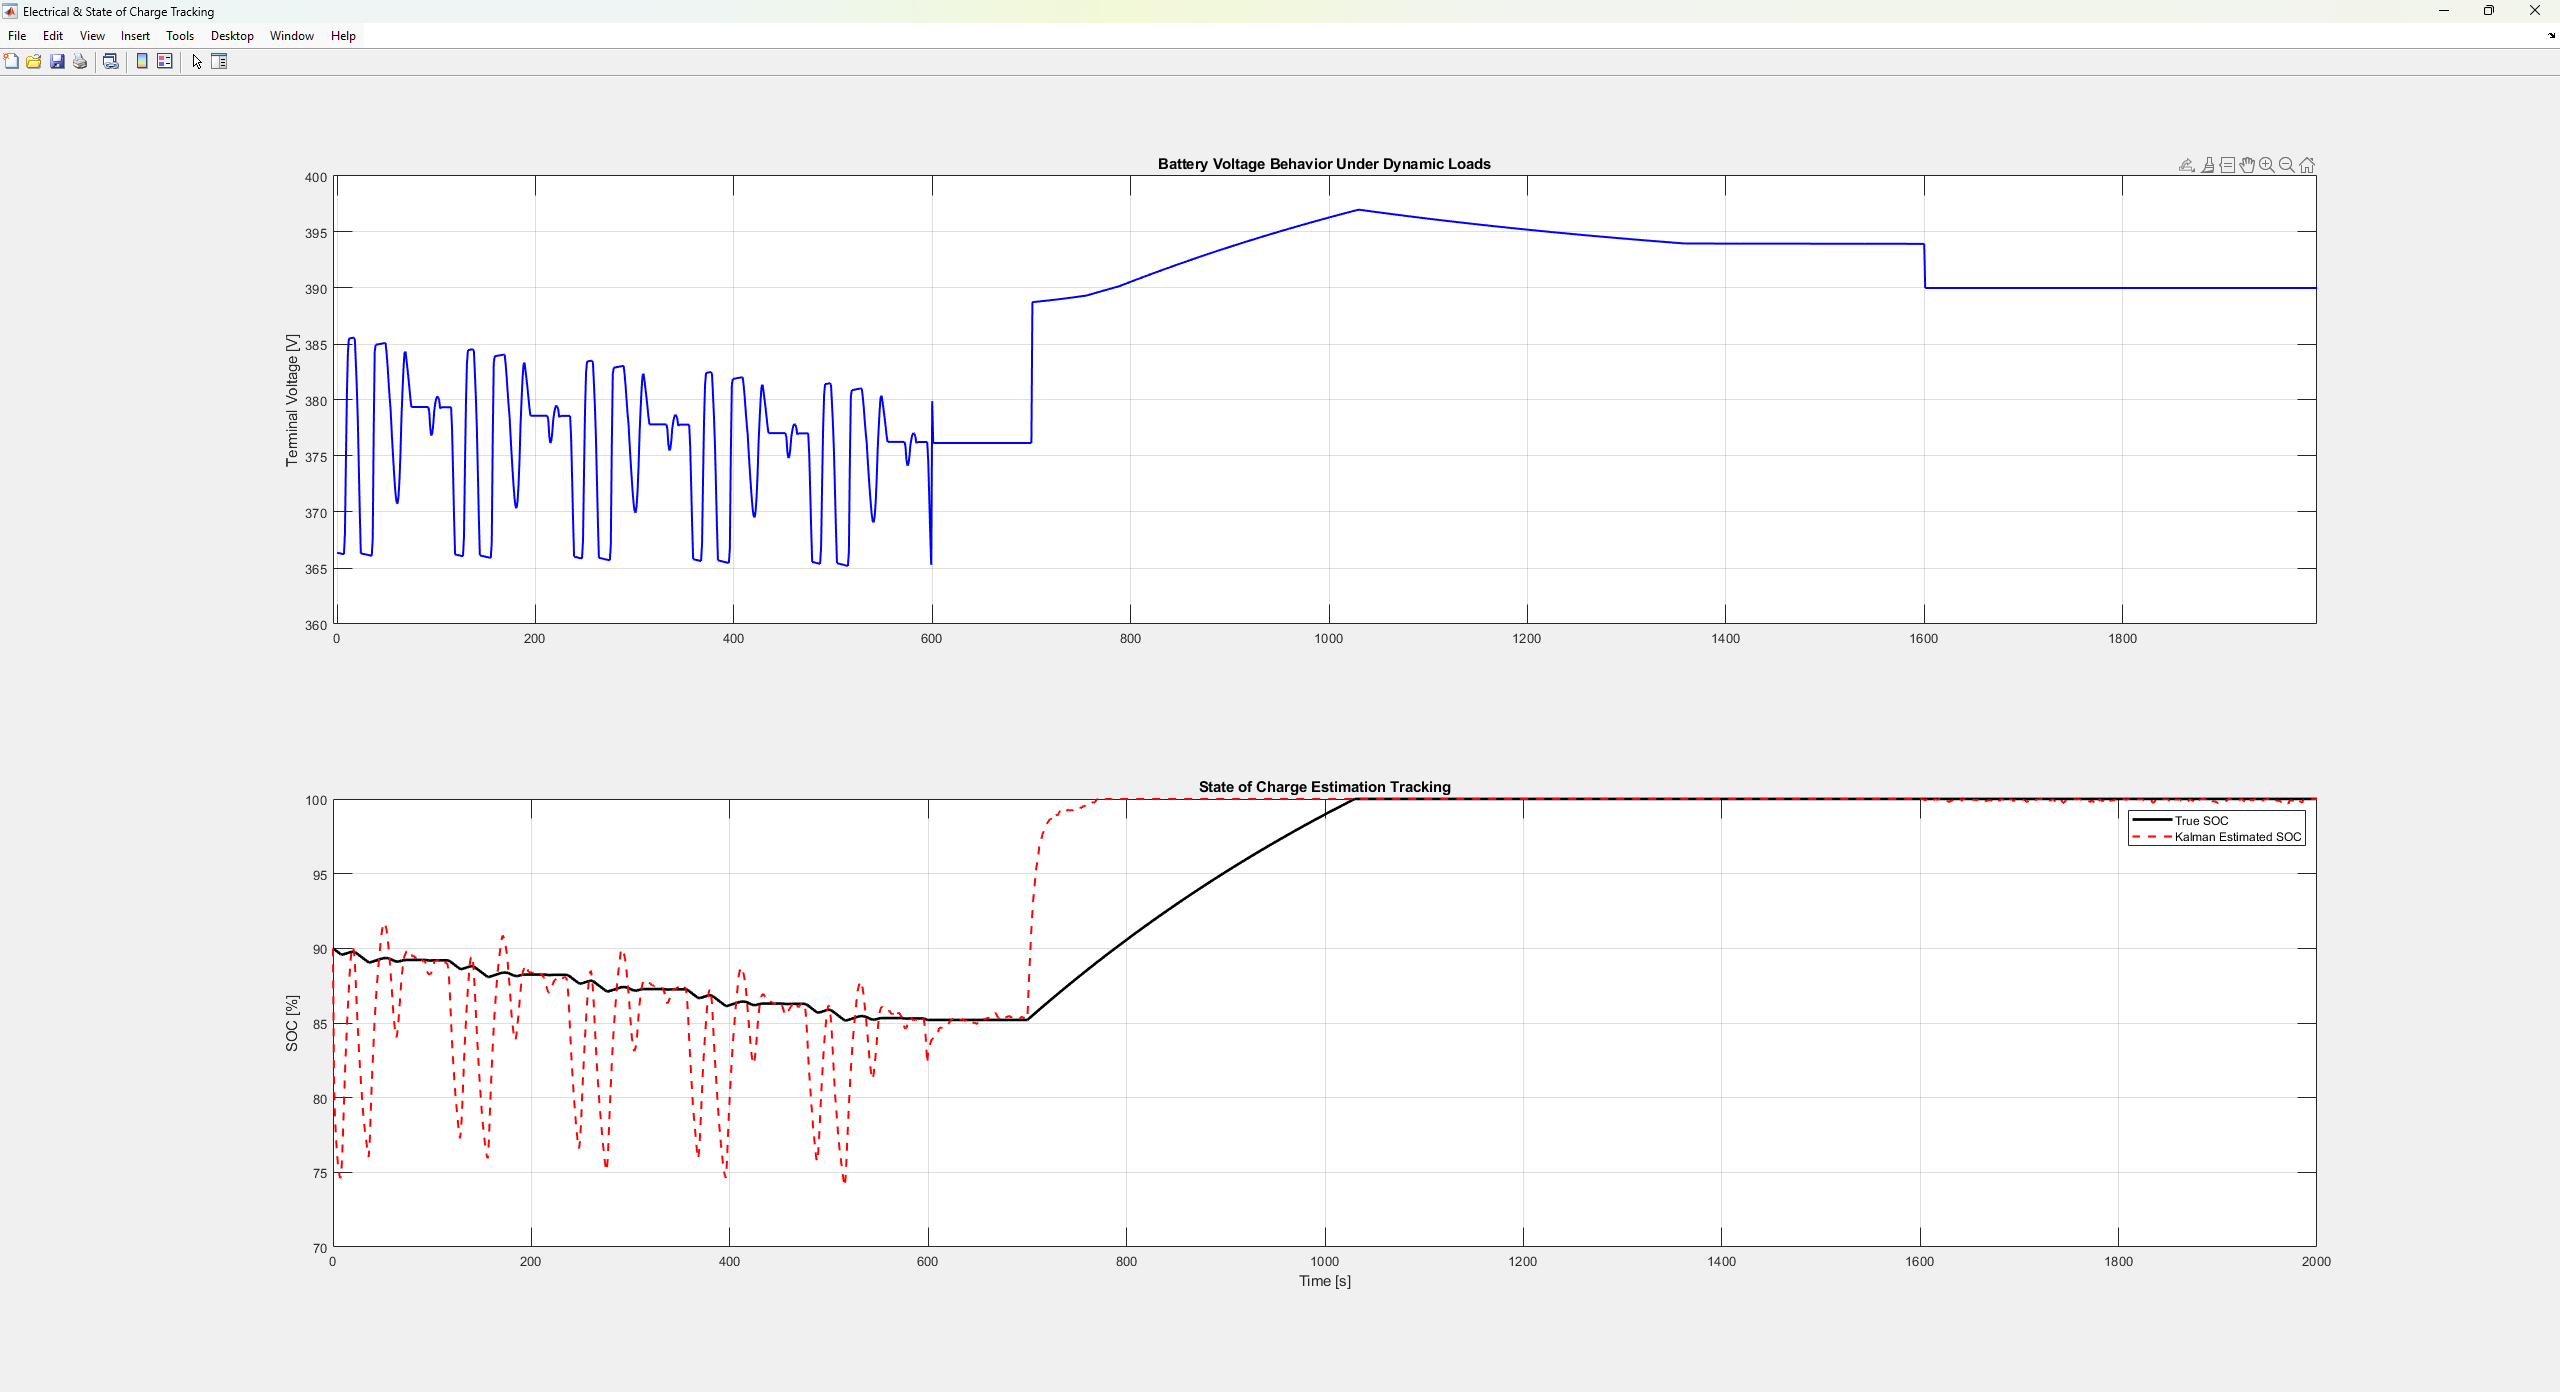
\includegraphics[width=0.95\linewidth]{Electrical_and_State_of_Charge_Tracking.png}
\caption{Battery terminal voltage and Kalman-filter SOC estimation vs.\ true SOC over the stress scenario.}
\label{fig:soc}
\end{figure}

\section{Discussion}
\label{sec:discussion}

The central finding of this work is that the brief's own question -- ``calculate energy-efficiency gains, predictive versus reactive'' -- does not have a universally positive answer, and reporting it as if it did would misrepresent the result. In the aggressive stress scenario, forecast-aware control does not save energy; it spends 11--13\% more cooling energy than the reactive baseline while eliminating every safety-threshold violation and reducing modelled aging by up to 7.7\%. This is consistent with the mechanism described by Zhang et al.~\cite{zhang2018} and the broader MPC thermal-management literature: predictive controllers convert a scheduling problem (when to spend cooling energy) into an optimisation problem, and the optimal schedule is not always the cheapest one in aggregate energy, particularly under a stress scenario engineered to combine driving and charging heat simultaneously.

The UDDS-based reactive-baseline diagnostics (Section~\ref{sec:results}, above) suggest this trade-off is scenario-dependent rather than fixed: on a milder, purely urban drive cycle, the reactive controller's threshold is never even triggered, meaning there is no energy expenditure to compare against and no safety margin at risk. A scenario of intermediate severity -- heavier urban driving or a moderate fast-charge event without the full aggressive stress test -- is the natural next experiment for establishing where, if anywhere, the energy trade-off reverses in the predictive controllers' favour.

The relative ordering between the predictive-lookahead and MPC controllers is also informative. Despite MPC's higher computational cost (a constrained nonlinear program solved every timestep, versus simple threshold and forecast-mean arithmetic for the predictive controller), MPC achieves the lowest actuator chatter of all three controllers because slew-rate penalisation is an explicit term in its cost function rather than an emergent property of a rule-based schedule. This suggests that in applications where compressor or pump wear is a binding constraint, MPC's benefit may lie less in energy or peak-temperature performance -- where the simpler predictive controller is already competitive -- and more in actuator longevity.

\section{Debugging and Validation}
\label{sec:debug}

Several cross-domain signal-alignment issues were found and corrected during development, applying the same diagnostic rigor as the reference thermal-modelling literature~\cite{huria2012}:

\begin{itemize}
\item \textbf{Ambient-temperature unit mismatch.} Early diagnostics compared a Celsius battery-temperature trace against an ambient signal still in Kelvin, producing an artificially large apparent self-heating rise ($\sim$8.7\textdegree C). Fixed by standardising on the actual Kelvin ambient timeseries and converting explicitly once before any subtraction.
\item \textbf{Time-vector mismatch.} Battery logging and ambient input did not share identical sample times. Fixed by restricting both signals to their common interval and interpolating before computing $\Delta T$.
\item \textbf{Workspace-clobbering ordering bug.} Running the MATLAB stress-scenario script after the UDDS signal-generation script silently overwrote the UDDS-based \texttt{Q\_heat\_ts}/\texttt{T\_amb\_ts} base-workspace variables with the synthetic scenario's data, causing the Simscape plant to simulate against the wrong input. This was traced by cross-checking two independently-computed numbers against each other -- an actively-cooled plant cannot run hotter than its own uncooled estimate, yet an early result appeared to show exactly that -- and fixed by reordering the pipeline so UDDS signal generation runs immediately before any Simscape simulation step, with nothing able to overwrite the workspace in between.
\item \textbf{Simulink model-rewiring bug.} Programmatically swapping the reactive controller block for a \texttt{matlab.System} predictive/MPC controller left a stub on one branch of the deleted block's output line, causing subsequent \texttt{add\_line} calls to fail with ``the destination port already has a line connection.'' Fixed by defensively clearing any existing line on each destination port before rewiring, regardless of the underlying cause.
\end{itemize}

The workspace-clobbering bug in particular illustrates a broader validation principle applied throughout this work: a numerically plausible result is not necessarily a physically consistent one, and cross-checking independently-derived quantities against each other -- here, an actively-cooled temperature against its own uncooled upper bound -- is what actually exposed the error, rather than any single diagnostic in isolation.

\section{Limitations and Future Work}
\label{sec:limitations}

Three limitations are noted for transparency. First, the predictive and MPC controllers have been validated on the lumped MATLAB thermal plant but not yet on identical Simscape Fluids physics; \texttt{matlab.System} implementations exist and build successfully into Simscape variants, but end-to-end simulation of those variants has not yet completed cleanly, and is the highest-priority remaining item. Second, exact signal logging for the UDDS reactive-baseline results (Section~\ref{sec:results}, above) is not currently configured in the Simscape model; the reported values are read from the model's scope trace rather than an exported \texttt{.mat} file, and enabling proper logging would allow that table to cite exact rather than visually-read values. Third, the predictive-lookahead controller's Simscape port uses only its heat-generation-forecast branch, since the plant driven by the UDDS scenario has no route-position or throttle signal to drive the charger-proximity or throttle-lookahead branches used in the MATLAB-only stress-scenario comparison.

Future work should prioritise completing the Simscape-side validation of all three controllers on identical plant physics, capturing exact benchmark tables for that comparison, and testing an intermediate-severity scenario to determine whether the energy trade-off identified in Section~\ref{sec:discussion} reverses under less extreme conditions than the current stress test.

\section{Conclusion}
\label{sec:concl}

This work presents a complete solution to the MathWorks ``Predictive Electric Vehicle Cooling'' Challenge Project: a Simscape Fluids battery cooling plant validated against a real EPA UDDS drive cycle, and three controllers -- reactive, predictive-lookahead, and constrained nonlinear MPC -- benchmarked against each other and an uncooled reference on an aggressive-drive and fast-charge stress scenario. The predictive and MPC controllers eliminate all safety-threshold temperature excursions the reactive baseline exhibits and reduce modelled battery aging by up to 7.7\%, at the cost of higher proactive cooling energy expenditure -- a genuine trade-off rather than an unconditional improvement, and one that appears to depend on scenario severity. Battery SOC is estimated via a Kalman filter, and an Arrhenius SEI-growth model translates thermal exposure into relative battery-aging and range impact, directly addressing the brief's advanced-work request.

\begin{thebibliography}{9}

\bibitem{mathworks_hub}
MathWorks, ``Predictive Electric Vehicle Cooling,'' \emph{MATLAB and Simulink Challenge Project Hub}, \url{https://github.com/mathworks/MATLAB-Simulink-Challenge-Project-Hub/tree/main/projects/Predictive\%20Electric\%20Vehicle\%20Cooling}.

\bibitem{huria2012}
T.~Huria, M.~Ceraolo, J.~Gazzarri, and R.~Jackey, ``High fidelity electrical model with thermal dependence for characterization and simulation of high power lithium battery cells,'' in \emph{2012 IEEE International Electric Vehicle Conference}, 2012, doi: 10.1109/IEVC.2012.6183271.

\bibitem{zhang2018}
Q.~Zhang et al., ``Two-Layer Model Predictive Battery Thermal and Energy Management Optimization for Connected and Automated Electric Vehicles,'' arXiv:1809.10002.

\bibitem{physinformed2026}
``Physics-Informed Predictive Control for Integrated Electric-Vehicle Thermal Management: An Open, Real-Data-Anchored Benchmark,'' arXiv:2606.22529.

\bibitem{hu2022}
L.~Hu, R.~Hu, Z.~Ma, and W.~Jiang, ``State of Charge Estimation and Evaluation of Lithium Battery Using Kalman Filter Algorithms,'' PMC9785816.

\bibitem{coulombkf2021}
``A Critical Look at Coulomb Counting Towards Improving the Kalman Filter Based State of Charge Tracking Algorithms in Rechargeable Batteries,'' arXiv:2101.05435.

\bibitem{chun2024}
H.~Chun et al., ``Comprehensive Study on Thermal Characteristics of Lithium-Ion Battery With Entropic Heat,'' \emph{International Journal of Energy Research}, 2024.

\bibitem{sei2012}
``Theory of SEI Formation in Rechargeable Batteries: Capacity Fade, Accelerated Aging and Lifetime Prediction,'' arXiv:1210.3672.

\bibitem{sei2020}
``Solid--Electrolyte Interphase During Battery Cycling: Theory of Growth Regimes,'' PMC7496968.

\bibitem{ramesh2015}
T.~N.~Ramesh and K.~V.~Rao, ``An Empirical Rate Constant Based Model to Study Capacity Fading in Lithium Ion Batteries,'' \emph{International Journal of Electrochemistry}, 2015.

\bibitem{smith2022}
K.~Smith et al., ``Lithium-Ion Battery Life Model with Electrode Cracking and Dead-Lithium Formation,'' NREL/TP-5700-79499, 2022.

\bibitem{coolingreview2024}
``A Review of Lithium-Ion Battery Thermal Management Based on Liquid Cooling and Its Evaluation Method,'' ResearchGate preprint, 2024.

\end{thebibliography}

\end{document}
